\chapter{Artifact Detection and Localization}

The artifact detection and localization pipeline is responsible for converting the sensor data from the various payloads (Mk. 0, Mk. 1, drone), into a list of artifacts to send to the base station and ultimately report to DARPA. The pipeline was developed to meet a set of requirements, which were derived from the competition rules and our team's concept of operations, shown in Table \ref{software_requirements}. Certain assumptions, given in Table \ref{software_assumptions} were made to constrain the scope of the problem and guide parameter tuning wherever necessary.

\begin{table}
	\centering
		\begin{adjustbox}{max width=.95\textwidth}
	\begin{tabular}{ |l| } 
	\hline
	Reported coordinate of artifact must be within 5m of DARPA-surveyed coordinate \\ \hline
	Pipeline must run on-board, either on the Xavier (Mk. 0, Mk. 1), or on part of the NUC (drone) \\ \hline
	Artifacts must be transmitted to base station reliably over a lossy wireless link \\  \hline
	Pipeline should be capable of detecting all 5 types of artifacts (as shown in Figure \ref{tunnel artifacts}) \\ \hline
	All artifacts which the robots pass by (within 5m) should be detected \\ \hline
	Pipeline should be identical or nearly identical on all payloads \\ \hline
	Artifacts should be detected and reported to human supervisor in real-time \\ \hline
\end{tabular}
\end{adjustbox}
\caption{Software pipeline requirements}
\label{software_requirements}
\end{table}

\begin{table}
	\centering
	\begin{adjustbox}{max width=.95\textwidth}
		\begin{tabular}{ |l| } 
			\hline
State estimation system on all payloads would be LOAM \cite{zhang2014loam} \\ \hline
Artifact detection and localization pipeline results would not feed the robots' waypoint planner \\ \hline 
Artifacts are reported in robots' own frames and transformed to a single world frame at base station \\ \hline
Robots will move at approximately 2 m/s \\ \hline
A human supervisor would be available to verify artifact reports, and thus false positives are acceptable \\ \hline
		\end{tabular}
	\end{adjustbox}
	\caption{Software pipeline assumptions}
	\label{software_assumptions}
\end{table}

An overview of the complete pipeline is given in Figure \ref{software_overview}. This pipeline runs identically on all 3 payloads with only minor configuration changes, and sensor omissions where necessary (e.g. drone payload does not contain a thermal camera). All robots report artifacts to the GUI independently, and no information is shared between pipelines running on individual payloads to prevent overloading the communication network.

\begin{figure}	
	\centering
	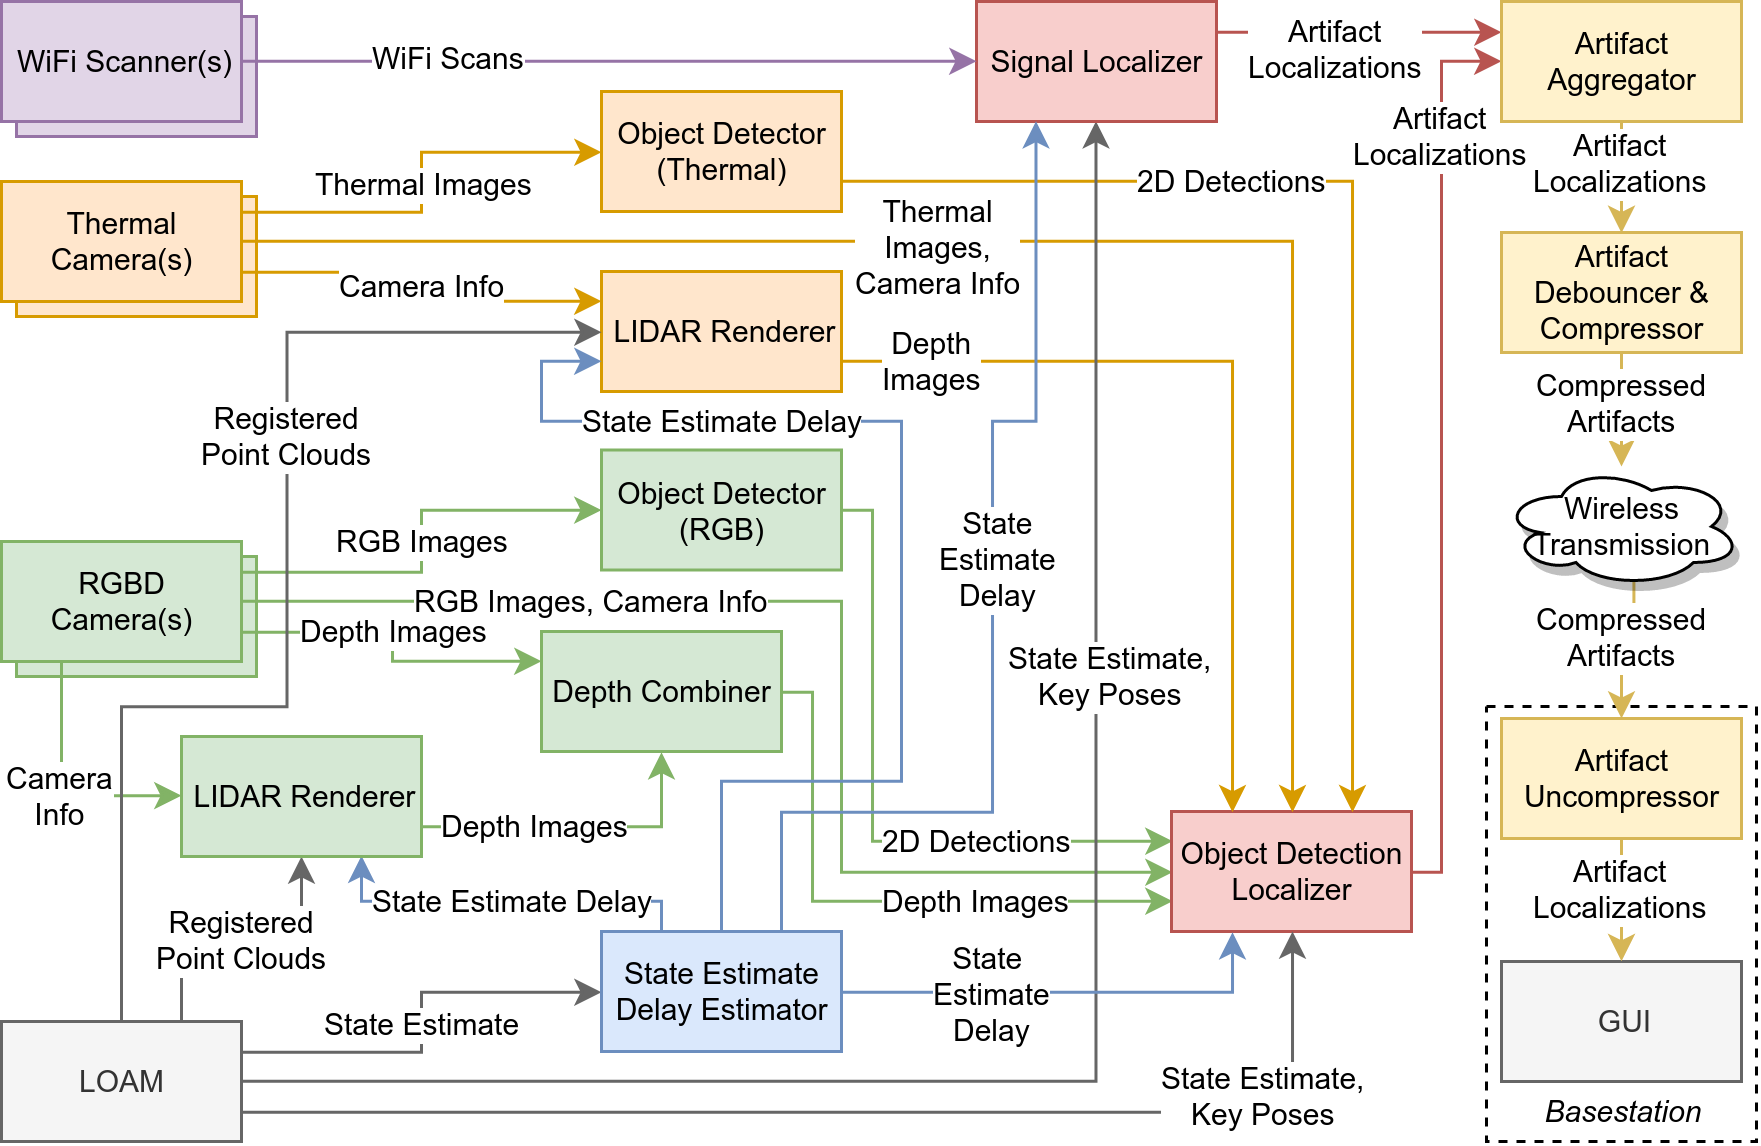
\includegraphics[width=\textwidth]{software_overview.png}
	\caption{Artifact detection and localization software diagram}
	\label{software_overview}
\end{figure}

The pipeline consists of 2 major modules - the Signal Localizer and the Object Detection Localizer. Each module takes in various sensor data and produces Artifact Localizations, which are 3D coordinates in the robot's map frame that are believed to correspond to a desired artifact. These Artifact Localizations may contain additional evidence to be displayed to the human supervisor, such as images or point clouds of the artifact and surrounding environment. The complete specification for an Artifact Localization message is given in Table \ref{artifact_localization}. Artifact Localizations from both modules are combined inside the Artifact Aggregator and then transmitted to the base station to be displayed on the GUI. The human supervisor inspects artifacts displayed on the GUI and reports valid ones to DARPA.

\begin{table}
	\centering
	\begin{adjustbox}{max width=.95\textwidth}
		\csvreader[
		respect underscore=true,
		tabular=|l|l|l|,
		late after line=\\\hline,
		% This is a terrible hack to get the multiline support I want.
		table head=\hline \textbf{Datatype} & \textbf{Field Name} & \textbf{Description}\\\hline,
		]{artifact_localization.csv}{}{\csvlinetotablerow}
	\end{adjustbox}
	\caption{Composition of an Artifact Localization message}
	\label{artifact_localization}
\end{table}

\section{LOAM Overview}

One of the assumptions made during the initial design phases of the software pipeline was that LOAM \cite{zhang2014loam} would be the state estimation system used on all of our payloads. This simplified the development of the artifact detection and localization pipeline as we only needed to develop and test against a single state estimation system. The relevant interface details of LOAM (in the form of ROS \cite{quigley2009ros} frames and topics) are given below:

\begin{description}
	\item[/sensor] This is the robot's local frame, and is coincident with the Velodyne LIDAR's frame.
	\item[/sensor\_init] The fixed frame used as the base for LOAM's odometry.
	\item[/map] The world frame, which is initially coincident with sensor\_init but can change after loop closures.
	\item[/key\_pose\_to\_map] LOAM creates a series of key poses as the robot traverses the environment. These key poses are generated approximately every 2 meters of the robot's path. Each key pose is given a unique ID, starting from 0. The key pose is published relative to the /map frame.
	\item[/key\_pose\_path] When LOAM detects a loop closure, it corrects the key poses and publishes a new list of key pose IDs and poses.
	\item[/velodyne\_cloud\_registered] The laser scan from the Velodyne LIDAR is aligned to previous scans and published on this topic at 5 Hz. Registered scans are published on this topic even when the robot is stationary. The scans are registered in the /sensor\_init frame and accumulate drift over time, but are locally smooth.
	\item[/integrated\_to\_map] The 6DOF pose of the /sensor frame is published on this topic at 200 Hz. The pose is corrected by loop closures and thus does not accumulate significant drift, but may be discontinuous locally.
\end{description}

\section{Object Detector (RGB)}

A 2D convolutional neural network based object detector runs on each of the RGB image stream to detect all artifact types except cell phones. To select the network, a variety of network architectures were benchmarked, identifying networks which would be capable of running at camera framerate on the NUC (for 1 RGB image stream) and on the Xavier (for 4 RGB image streams). Pretrained checkpoints for the fastest network types were finetuned using manually collected and annotated data. The best performing networks were selected for use in the pipeline.

The TensorFlow Object Detection API \cite{huang2017speed} was used for all network training and inference tasks. The API provides checkpoints for a large variety of popular network architectures, and has support from both Nvidia and Intel for optimizing networks trained with the API to run on their respective hardware platforms. The YOLO \cite{redmon2018yolov3} family of networks was not considered for use in the Artifact Detection and Localization pipeline due to the lack of support for it in the API.

\subsection{Network Benchmarking and Selection}

The TensorFlow Object Detection API was used to evaluate a large number of network architectures and configurations for inference speed on the Nvidia Xavier and Intel NUC. All models available in the model zoo were downloaded, optimized for each hardware platform, and benchmarked for average inference speed. 

\subsubsection{Xavier Benchmarks}

Nvidia provides the TensorRT runtime to accelerate neural network inference on its platforms. Using the TensorRT runtime directly is typically a difficult and involved process. TF-TRT bindings are provided within TensorFlow to simplify the use of TensorRT for certain types of models trained with TensorFlow. After converting a network from TensorFlow to TF-TRT, supported subgraphs of the network will be converted into optimized TensorRT engines, while unsupported operations will execute natively in TensorFlow. Support is provided by Nvidia for models trained with the TensorFlow Object Detection API to ensure many model types can be converted using TF-TRT. 

During conversion, all networks were optimized to use 16 bit floating precision, which typically achieves comparable network precision and accuracy as 32 bit precision while allowing for higher inference throughput. Batch sizes of 1 and 4 were used, representing configurations where images from each camera are processed sequentially, or a batch of images (one from each camera) is processed at once. A minimum segment size of 50 was used. Some networks failed to convert to TF-TRT with these parameters and were ignored. Before benchmarking, all CPU and GPU cores on the Xavier were enabled (MAX-N mode) and had their frequency maximized. The fan was set to run at maximum speed to prevent overheating during test runs. 

When benchmarking a network, a set of images (equivalent to the network's batch size) was first run through it to allow TensorFlow to optimize runtime parameters. The same set of images were then run through the network 100 times in a loop, and the inference times for each loop iteration were recorded. No limits were placed on the number of cores, percent of GPU, or percent of system memory available to the neural network. The average of the loop iteration times are presented in Table \ref{trt_graphs} for each network architecture which was successfully converted with TF-TRT. Table \ref{reference_graphs} shows the average loop iteration time for all unoptimized networks as a baseline, including networks which were unable to be converted.

% https://tex.stackexchange.com/questions/97505/shrink-table-to-fit-on-a-page-or-keep-it-as-it-is
% https://tex.stackexchange.com/questions/269545/csvreader-and-respect-all-special-characters-in-the-csv-file	

\begin{table}
	\centering
	\begin{adjustbox}{max width=.95\textwidth}
		\csvreader[
		respect underscore=true,
		tabular=|c|c|c|c|,
		late after line=\\\hline,
		% This is a terrible hack to get the multiline support I want.
		table head=\hline & \textbf{Batch} & \textbf{Average Batches} & \textbf{Average Frames} \\
		\textbf{Model Checkpoint Name} & \textbf{Size} & \textbf{Per Second} & \textbf{Per Second}\\\hline,
		% table head=\hline \textbf{Model Checkpoint Name} & \textbf{Batch Size} & \textbf{Average Batches per Second} & \textbf{Average Frames per Second}\\\hline,
		]{trt_graphs.csv}{}{\csvlinetotablerow}
	\end{adjustbox}
	\caption{Optimized TF-TRT network inference benchmarks on Xavier}
	\label{trt_graphs}
\end{table}

\begin{table}
	\centering
	\begin{adjustbox}{max width=.95\textwidth}
		\csvreader[
			respect underscore=true,
			tabular=|c|c|c|c|,
			late after line=\\\hline,
			% This is a terrible hack to get the multiline support I want.
			table head=\hline & \textbf{Batch} & \textbf{Average Batches} & \textbf{Average Frames} \\
						\textbf{Model Checkpoint Name} & \textbf{Size} & \textbf{Per Second} & \textbf{Per Second}\\\hline,
			% table head=\hline \textbf{Model Checkpoint Name} & \textbf{Batch Size} & \textbf{Average Batches per Second} & \textbf{Average Frames per Second}\\\hline,
		]{reference_graphs.csv}{}{\csvlinetotablerow}
	\end{adjustbox}
	\caption{Reference network inference benchmarks on Xavier}
	\label{reference_graphs}
\end{table}

The values reported in Table \ref{trt_graphs} were gathered after optimizing and benchmarking each network once. Repeated benchmarking attempts resulted in very similar average frames per second values. However, repeatedly rerunning the optimization process with TF-TRT and then benchmarking each network resulted in some deviation from the observed average frames per second values, up to approximately 25\% from those reported in Table \ref{trt_graphs}. Thus, the average frames per second values reported in Table \ref{trt_graphs} are not necessarily the maximum possible framerates under the optimization parameters, but we believe they are sufficiently close to inform network selection.

\subsubsection{NUC Benchmarks}

Intel provides the OpenVINO framework which serves a similar purpose as TensorRT on Nvidia's platforms. While no dedicated integration with TensorFlow is available for OpenVINO, specific examples are provided by Intel on optimizing networks trained with the TensorFlow Object Detection API with the OpenVINO framework. Using the available examples, most models based on SSD, FasterRCNN, and MaskRCNN were able to be converted into the intermediate representation used by OpenVINO. 32 bit floating point weights were used.

The models were benchmarked using a nearly identical process to the Xavier benchmarking. OpenVINO was only allowed to use one CPU core during benchmarking, representing a realistic upper bound on the compute available for network inference when other processes are running on the NUC. CPU frequencies were governed automatically. GPU support was not enabled for OpenVINO. Benchmarking results from successfully converted models are given in Table \ref{openvino_graphs}.

\begin{table}
	\centering
	\begin{adjustbox}{max width=.95\textwidth}
		\csvreader[
		respect underscore=true,
		tabular=|c|c|c|,
		late after line=\\\hline,
		% This is a terrible hack to get the multiline support I want.
		table head=\hline & \textbf{Batch} & \textbf{Average Frames} \\
		\textbf{Model Checkpoint Name} & \textbf{Size} & \textbf{Per Second}\\\hline,
		]{openvino_graphs.csv}{}{\csvlinetotablerow}
	\end{adjustbox}
	\caption{OpenVINO optimized network benchmarks on NUC (1 core)}
	\label{openvino_graphs}
\end{table}

\subsubsection{Network Selection}

The primary criteria for selecting a network architecture was the throughput. The relatively low framerate of the RGB cameras (a maximum of 15 Hz on Mk. 0) often causes motion blur, which negatively impacts detection performance. By ensuring that the selected network would be able to run on each frame, we would increase the probability of detecting objects. The SSD MobileNet v1 architecture with COCO 2018/01/28 checkpoint was selected as the base for all networks to run on the Xavier and NUC due to it offering the highest throughput on the Xavier (with a batch size of 4) and offering sufficiently fast throughput (>15 Hz) on the NUC.

Table \ref{trt_graphs} only gives benchmarks up to a batch size of 4. To investigate if additional throughput gains were possible for the selected network architecture, we benchmarked the network with larger batch sizes as well, as shown in Table \ref{batch_size_graphs}. Batch sizes larger than 4 would require sending more than one image per stream through the network at once. Table \ref{batch_size_graphs} indicates that this would increase throughput slightly, but it was decided that the added latency and complexity of batching multiple images per stream did not outweigh the small marginal increase in throughput as compared to using a single image per stream (with a batch size of 4).

\begin{table}
	\centering
	\begin{adjustbox}{max width=.9\textwidth}
		\csvreader[
		respect underscore=true,
		tabular=|c|c|c|c|c|,
		late after line=\\\hline,
		% This is a terrible hack to get the multiline support I want.
		table head=\hline & \textbf{Batch} & \textbf{Average Batches} & \textbf{Average Frames} & \textbf{Relative}\\
		\textbf{Model Checkpoint Name} & \textbf{Size} & \textbf{Per Second} & \textbf{Per Second} & \textbf{Speedup}\\\hline,
		% table head=\hline \textbf{Model Checkpoint Name} & \textbf{Batch Size} & \textbf{Average Batches per Second} & \textbf{Average Frames per Second}\\\hline,
		]{batch_size_graphs.csv}{}{\csvlinetotablerow}
	\end{adjustbox}
	\caption{Inference throughput with varying batch size on Xavier}
	\label{batch_size_graphs}
\end{table}

\subsection{Data Collection and Labeling}

To finetune the selected checkpoint for object detection in the Tunnel Circuit, a large dataset of images and bounding boxes was collected and manually annotated. The dataset contains images sampled from videos of all 5 categories of objects captured from handheld devices, the ground robots, and the drone, in a variety of environments and lighting conditions. Images were labeled using a combination of custom semi-automated and manual tooling.

\subsubsection{Data Collection}

The dataset used to train the network used during the Tunnel Circuit was trained on data collected from the environments listed in Table \ref{environment_descriptions}. A representative image for each environment can be seen in Figure \ref{environments}. Data was collected in each environment using either a custom handheld setup with a RealSense, thermal camera, and LEDs, or directly from the payloads on each robot. When collecting video of each artifact, only the exact model of artifact specified by DARPA was used as no generalization across different models of artifact was required for the Tunnel Circuit.

\begin{table}[]
	\centering
	\resizebox{.95\textwidth}{!}{
		\begin{tabular}{|l|l|}
			\hline
			\textbf{Environment Name} & \textbf{Environment Description}                                                   \\ \hline
			Gates Hallway             & The hallway outside Team Explorer's workspace at CMU in the Gates building         \\ \hline
			Gates Garage              & The parking complex attached to the Gates building (data collected at night)       \\ \hline
			Catacombs                 & Dusty underground storage area at CMU                                              \\ \hline
			Tour Ed Mine              & An old coal mine in Tarentum, PA where the majority of field testing was performed \\ \hline
			STIX Airbnb               & Trail outside the Airbnb Team Explorer stayed at in Colorado during the STIX event \\ \hline
			STIX Mine                 & The Edgar Experimental Mine where DARPA hosted the STIX event                      \\ \hline
		\end{tabular}%
	}
	\caption{List of environments where data was collected for the Tunnel Circuit dataset}
	\label{environment_descriptions}
\end{table}

\begin{figure}
	\centering
	\begin{subfigure}{0.3\textwidth}
		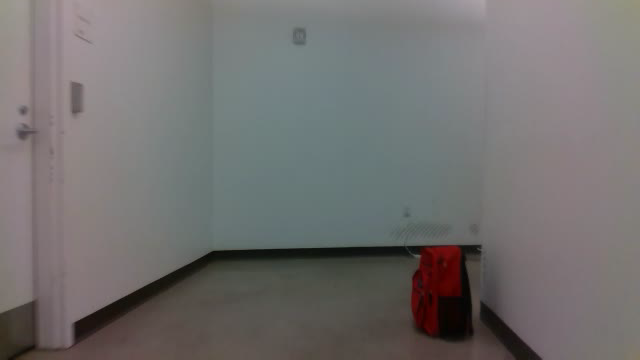
\includegraphics[width=\textwidth]{environments/hallway.png}
		\caption{Gates Hallway}
		\label{environment_hallway}
	\end{subfigure}		
	\hfill
	\begin{subfigure}{0.3\textwidth}
		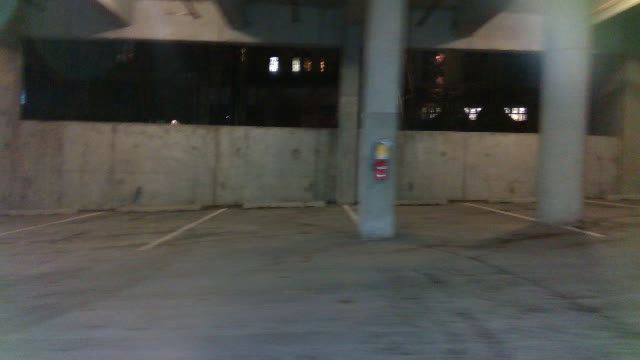
\includegraphics[width=\textwidth]{environments/gates.png}
		\caption{Gates Garage}
		\label{environment_gates}		
	\end{subfigure}
	\hfill
	\begin{subfigure}{0.3\textwidth}
		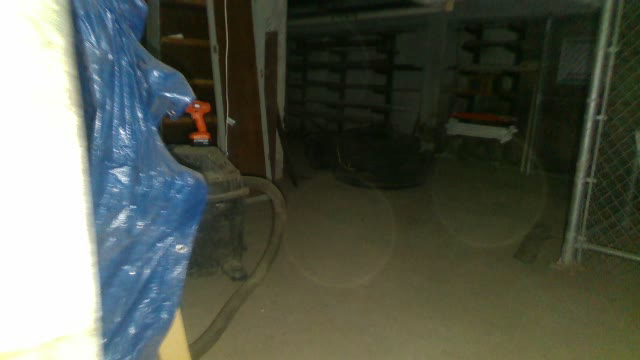
\includegraphics[width=\textwidth]{environments/catacombs.png}
		\caption{Catacombs}
		\label{environment_catacombs}
	\end{subfigure}
	\\
	\begin{subfigure}{0.3\textwidth}
		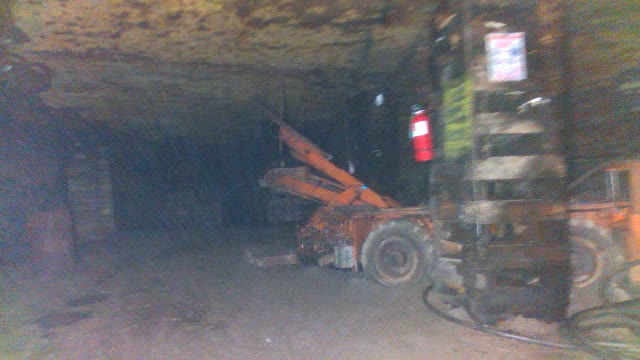
\includegraphics[width=\textwidth]{environments/tour_ed.png}
		\caption{Tour Ed Mine}
		\label{environment_tour_ed}
	\end{subfigure}		
	\hfill
	\begin{subfigure}{0.3\textwidth}
		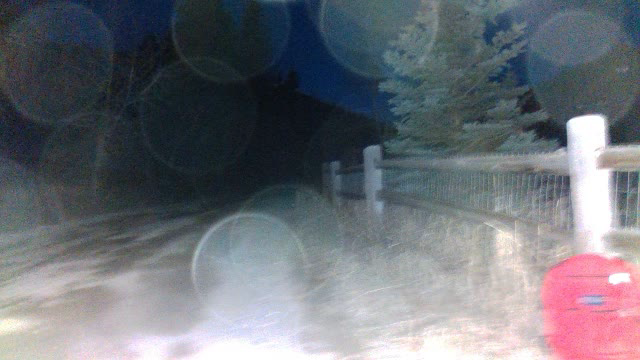
\includegraphics[width=\textwidth]{environments/colorado.png}
		\caption{STIX Airbnb}
		\label{environment_colorado}		
	\end{subfigure}
	\hfill
	\begin{subfigure}{0.3\textwidth}
		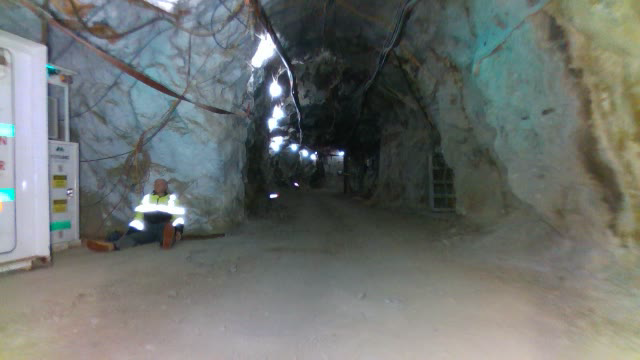
\includegraphics[width=\textwidth]{environments/stix.png}
		\caption{STIX Mine}
		\label{environment_stix}
	\end{subfigure}	
	\caption[Representative dataset collection environment images]{A representative image for each environment in the Tunnel Circuit dataset is shown in the Figure. All images except Figure \ref{environment_catacombs} were captured from payloads. Figure \ref{environment_catacombs} was captured with the handheld setup. Bokeh effects visible in Figure \ref{environment_catacombs} and Figure \ref{environment_colorado} are due to dust accumulation on the lens. Noise in Figure \ref{environment_tour_ed} is due to dust in the air being illuminated by the payload's bright LEDs.}
	\label{environments}
\end{figure}

Handheld data was collected by placing an artifact in a variety of locations and poses around the environment and recording short video clips while moving the handheld setup around. For each video clip, the cameras started recording when very close to the artifacts, and then moved backwards. The cameras were also moved around to capture a variety of viewpoints while ensuring that the artifact always stayed in frame. Video clips were typically less than 15 seconds long, and typically only had a single artifact visible at a time. It was assumed that this would be the case in the Tunnel Circuit due to the small number of artifacts (20) and large traversal distance (up to 4km). This assumption was not confirmed by DARPA. For safety, a small number of video clips were gathered with multiple artifacts in close proximity. 

Video from the payloads was collected by recording video feeds from all cameras on the robot during both autonomous exploration and teleoperation in the test environments. Teleoperation ensured that all artifacts in the environment would be seen by the robot and at a slow and smooth pace, while autonomous exploration generated data with realistic issues, such as motion blur and rolling shutter effects in a number of frames. Artifacts would be spread through the environment prior to the run and were not moved while data was being gathered. Payload videos typically exceeded 20 minutes each and only had artifacts visible in a small number of frames, but served as valuable source of realistic data and negative examples for the dataset.

\subsubsection{Data Labeling}

The video clips gathered from the handheld devices were collected in a way to be amenable to a semi-automatic data labeling based on image tracking. Using a custom labeling program, a human labeler draws and labels bounding boxes around each artifact. An image tracker is initialized for each individual bounding box, and is used to update the bounding box for each artifact in every frame. The human labeler presses a key to step through each frame and watches the automatically updated bounding boxes to ensure they are still sufficiently accurate. If the tracker fails for any reason, the labeler adjusts the bounding box to tightly bound the artifact again, and the tracker is reinitialized with the new box. The label assigned to the box is used throughout the entire video clip. Figure \ref{semi_automatic_labeling} shows frames labeled with this process sampled evenly from a 30 second video clip.

\begin{figure}
	\centering
	\begin{subfigure}{0.32\textwidth}
		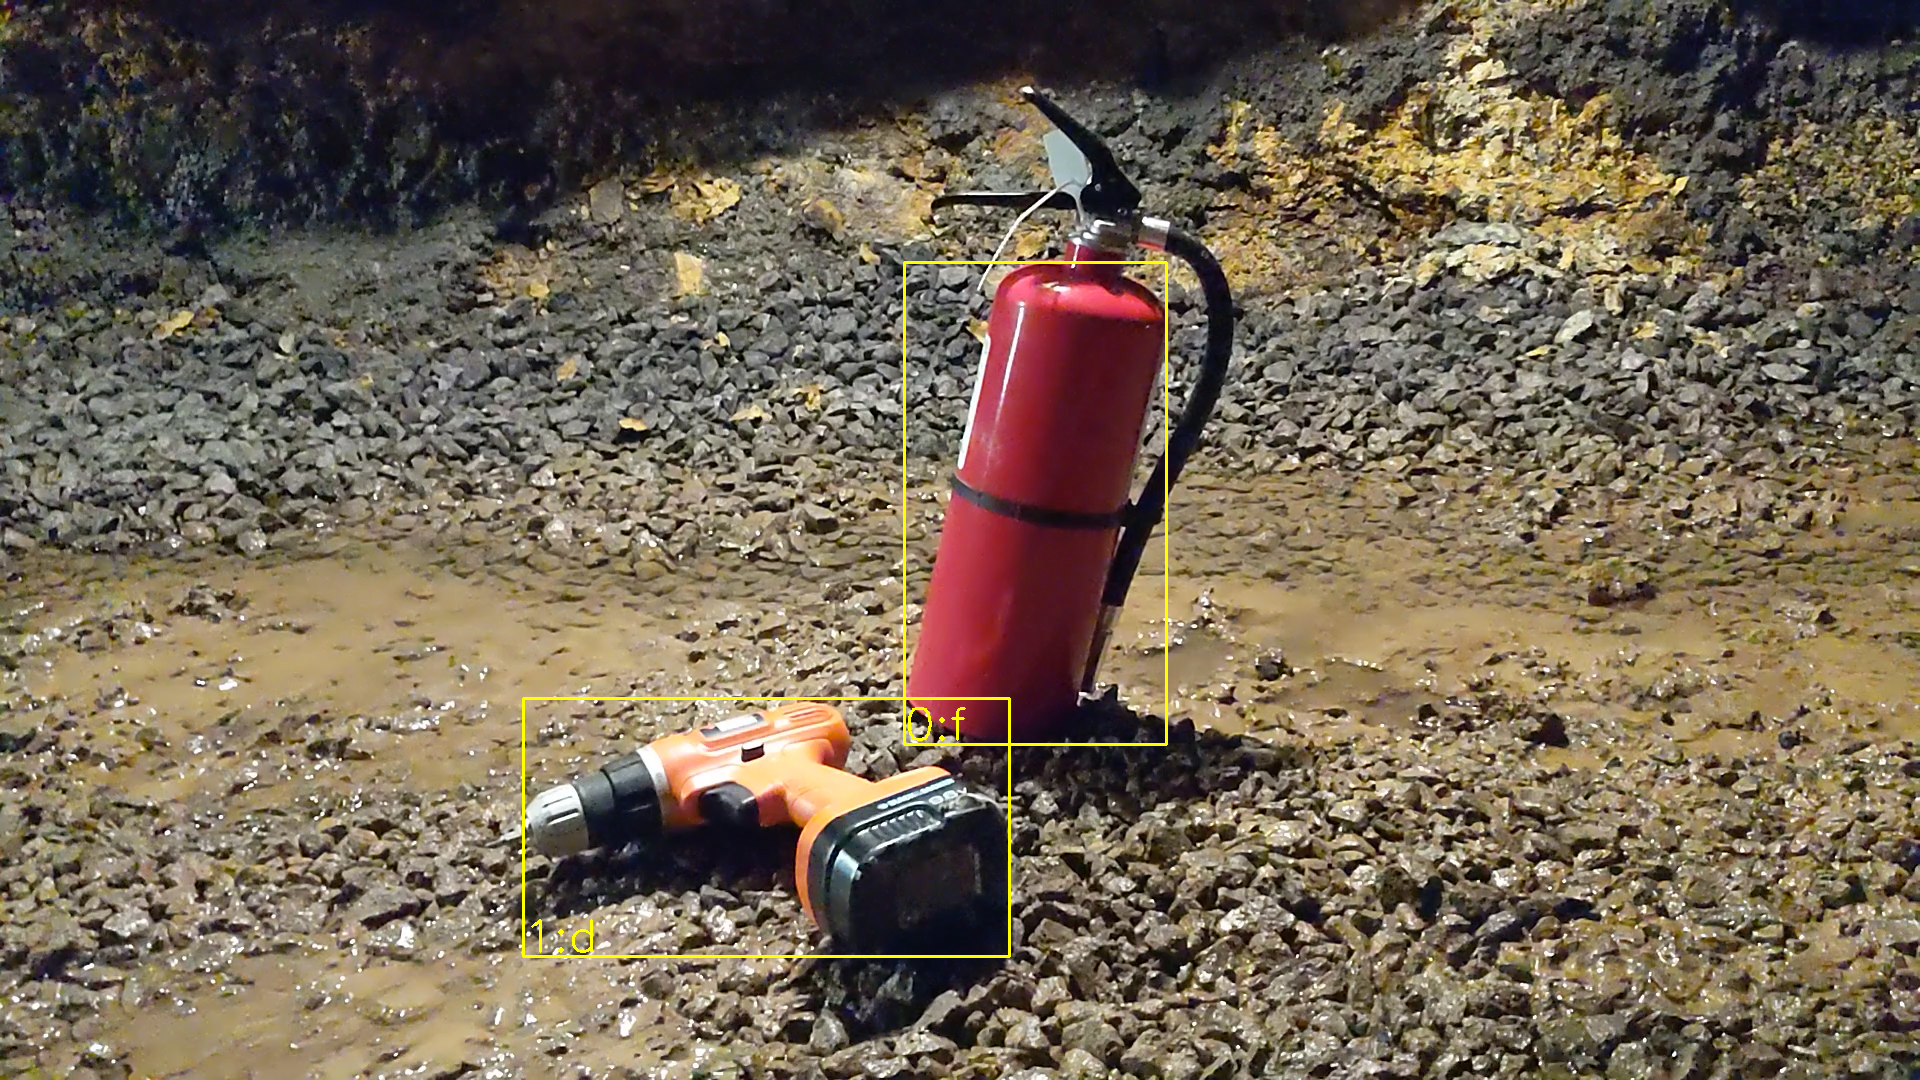
\includegraphics[width=\textwidth]{tracking/rect_00000.png}
	\end{subfigure}		
	\hfill
	\begin{subfigure}{0.32\textwidth}
		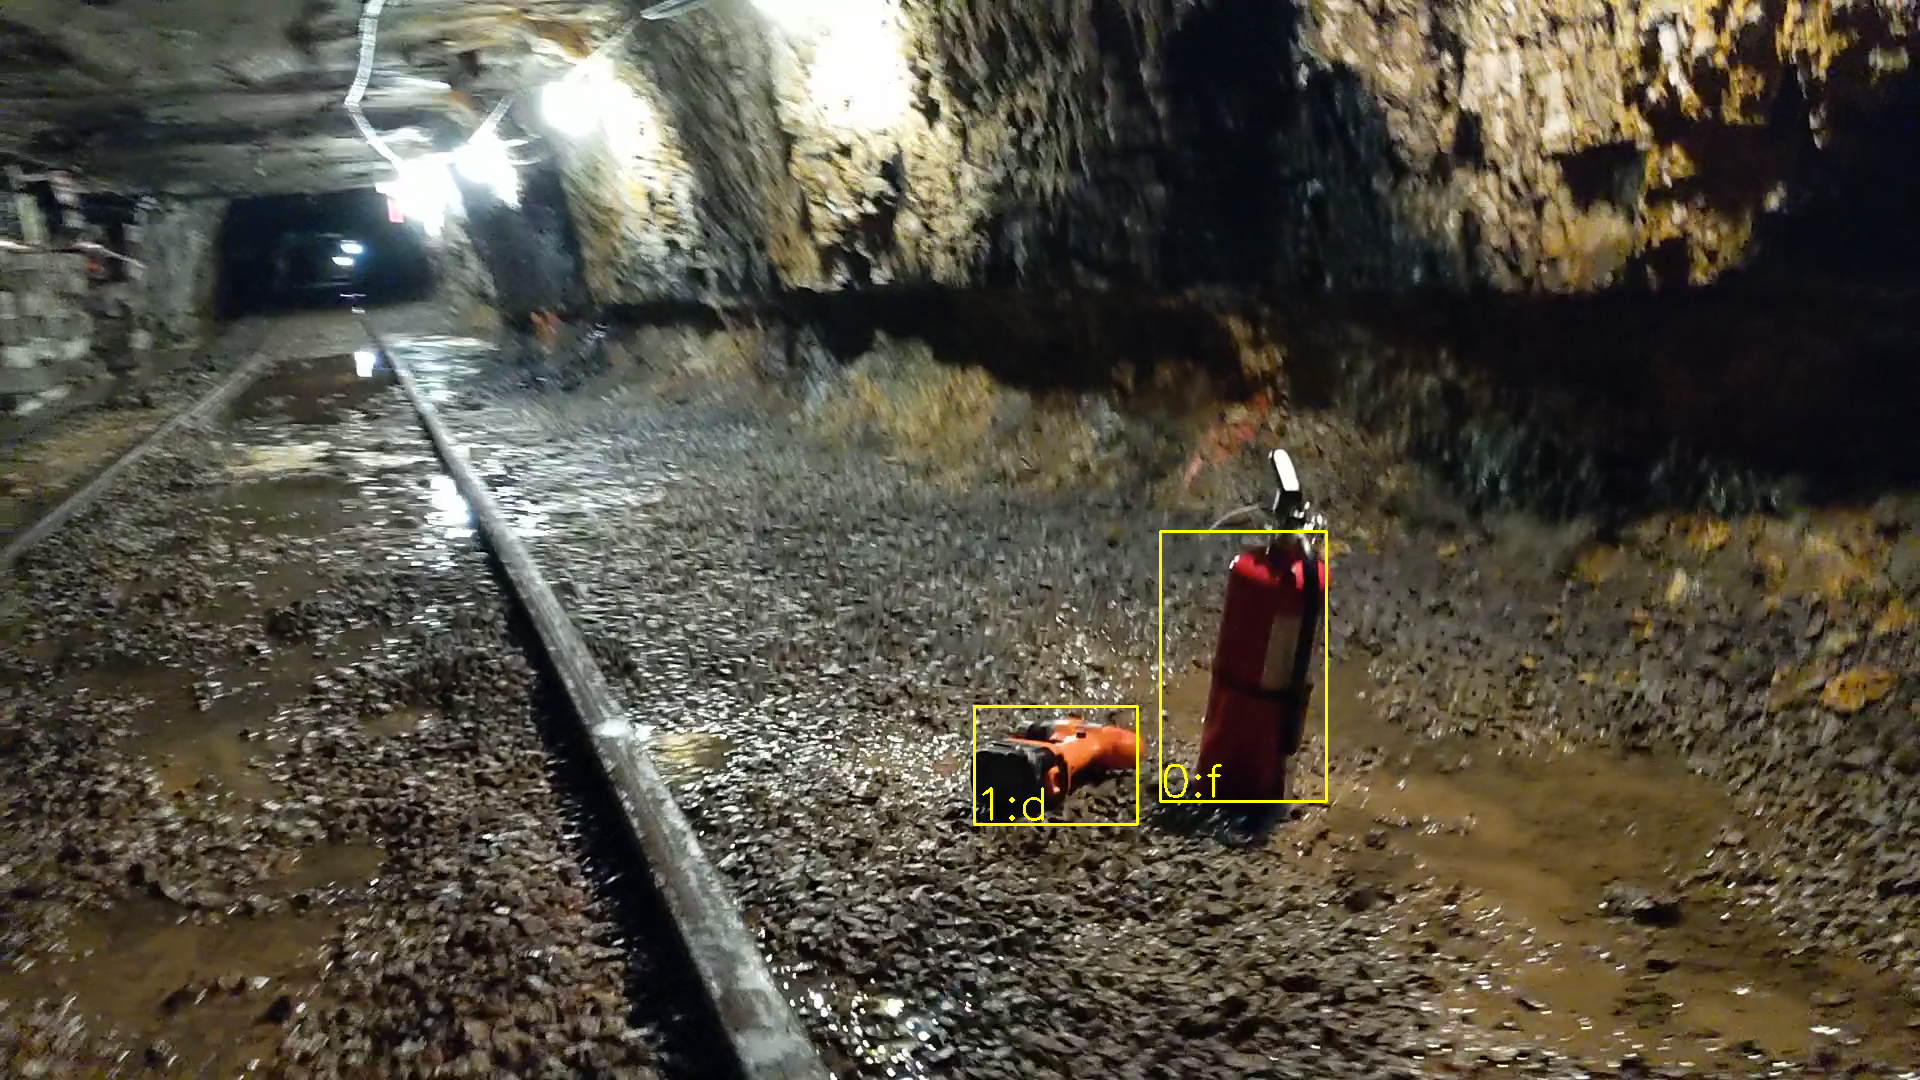
\includegraphics[width=\textwidth]{tracking/rect_00180.png}
	\end{subfigure}
	\hfill
	\begin{subfigure}{0.32\textwidth}
		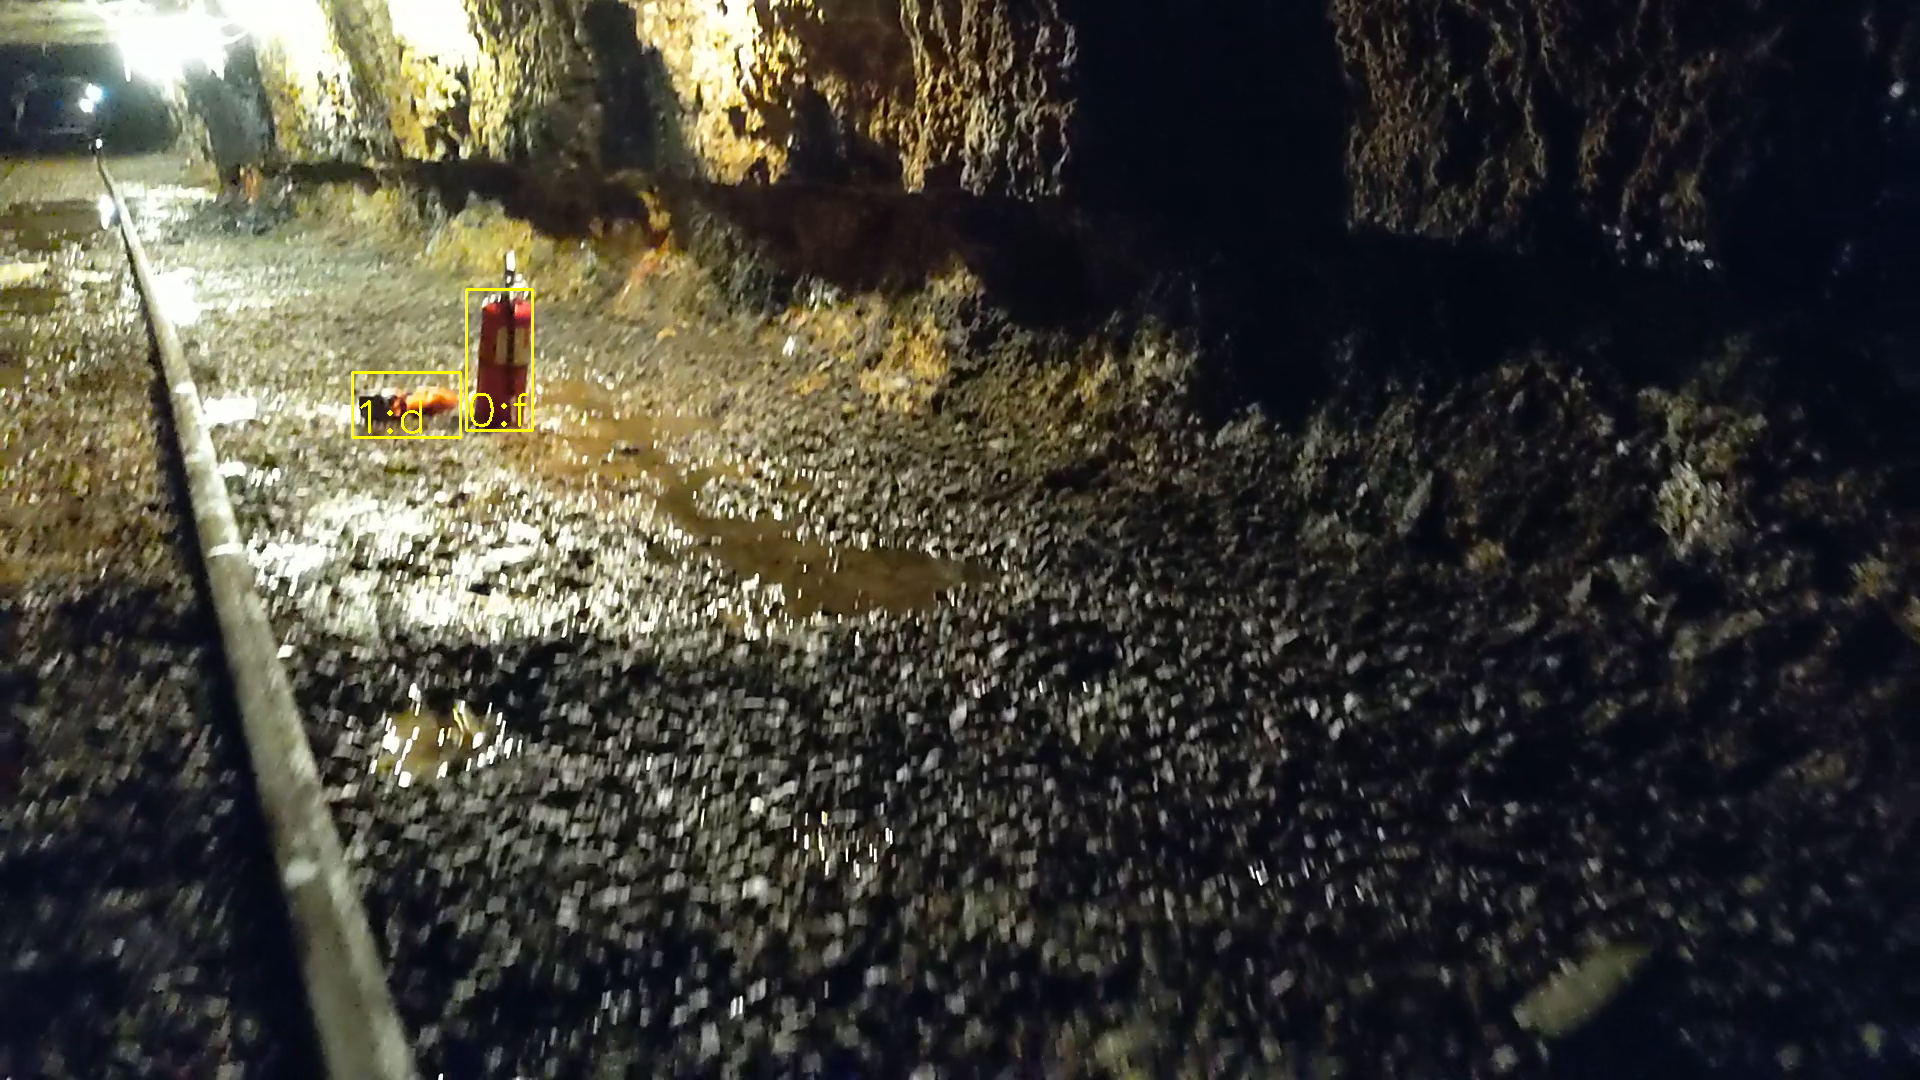
\includegraphics[width=\textwidth]{tracking/rect_00360.png}
	\end{subfigure}
	\\
	\begin{subfigure}{0.32\textwidth}
		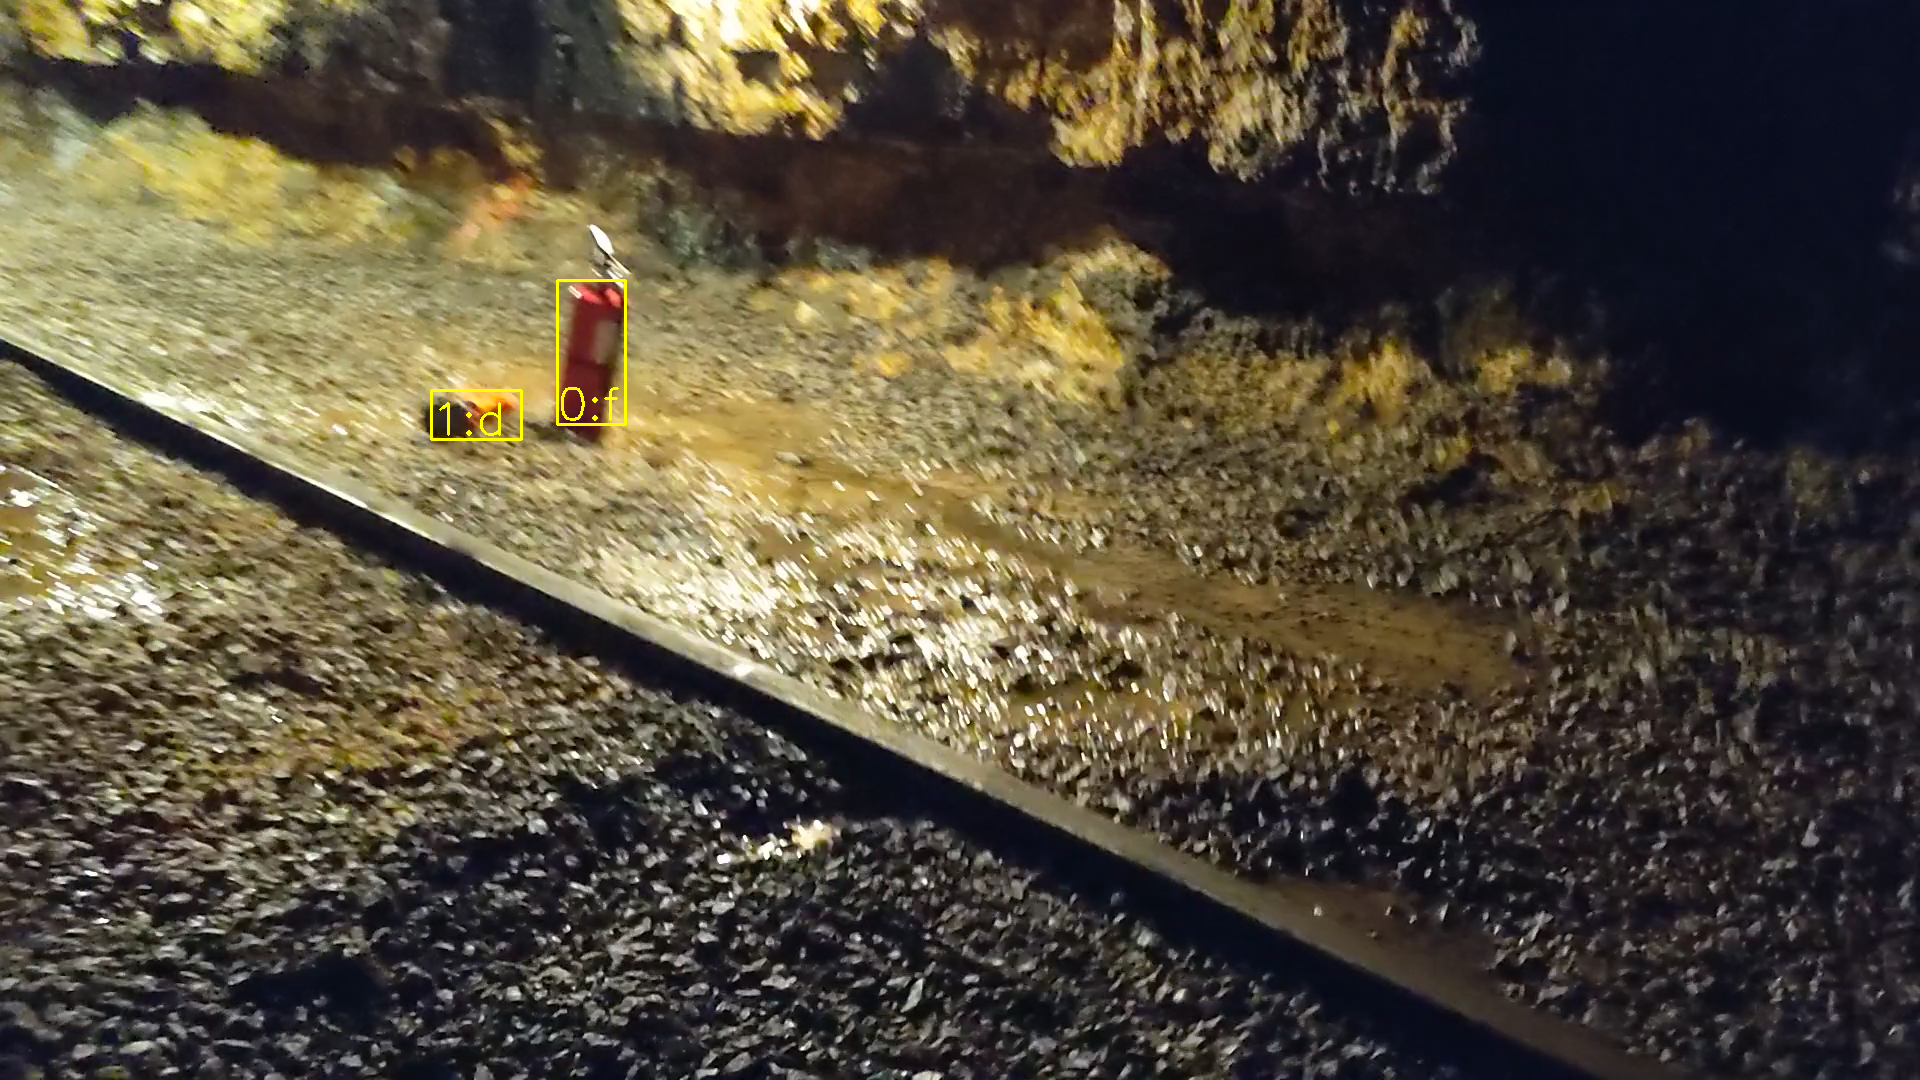
\includegraphics[width=\textwidth]{tracking/rect_00540.png}
	\end{subfigure}		
	\hfill
	\begin{subfigure}{0.32\textwidth}
		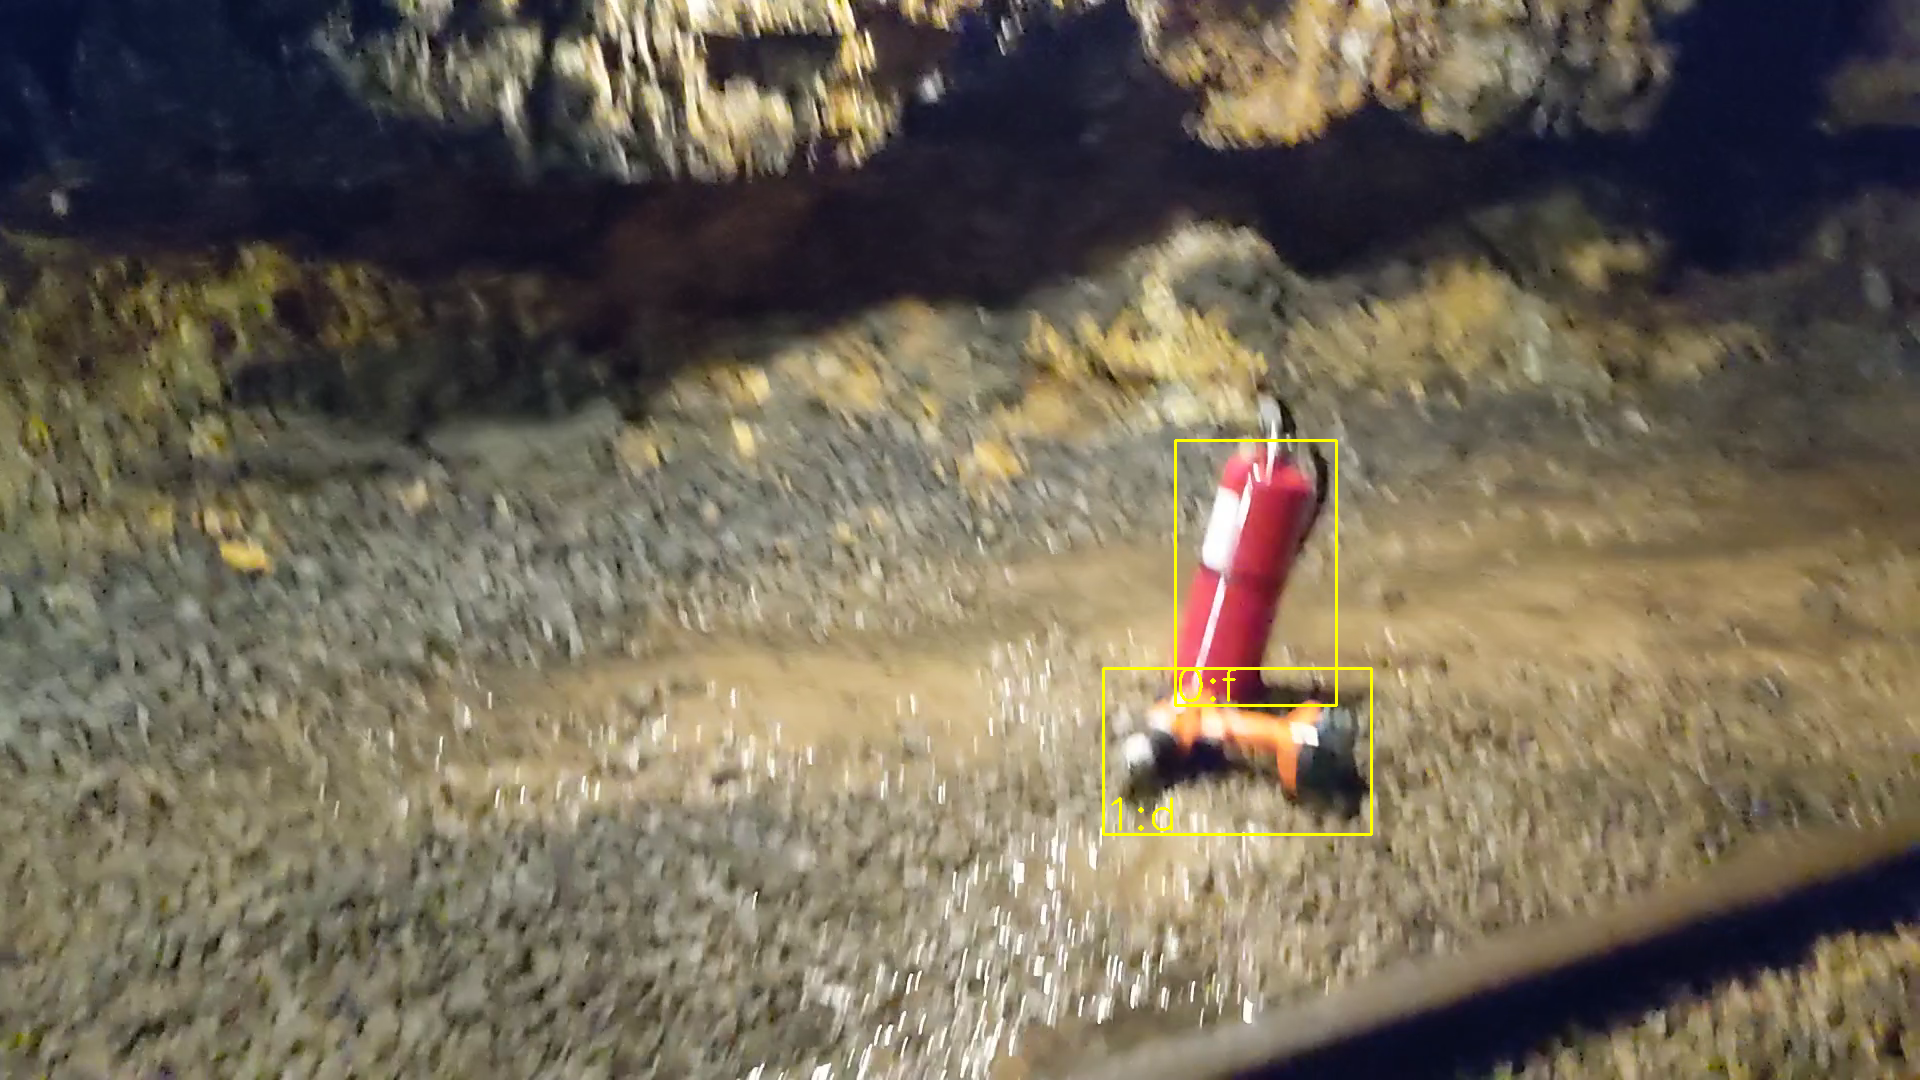
\includegraphics[width=\textwidth]{tracking/rect_00720.png}
	\end{subfigure}
	\hfill
	\begin{subfigure}{0.32\textwidth}
		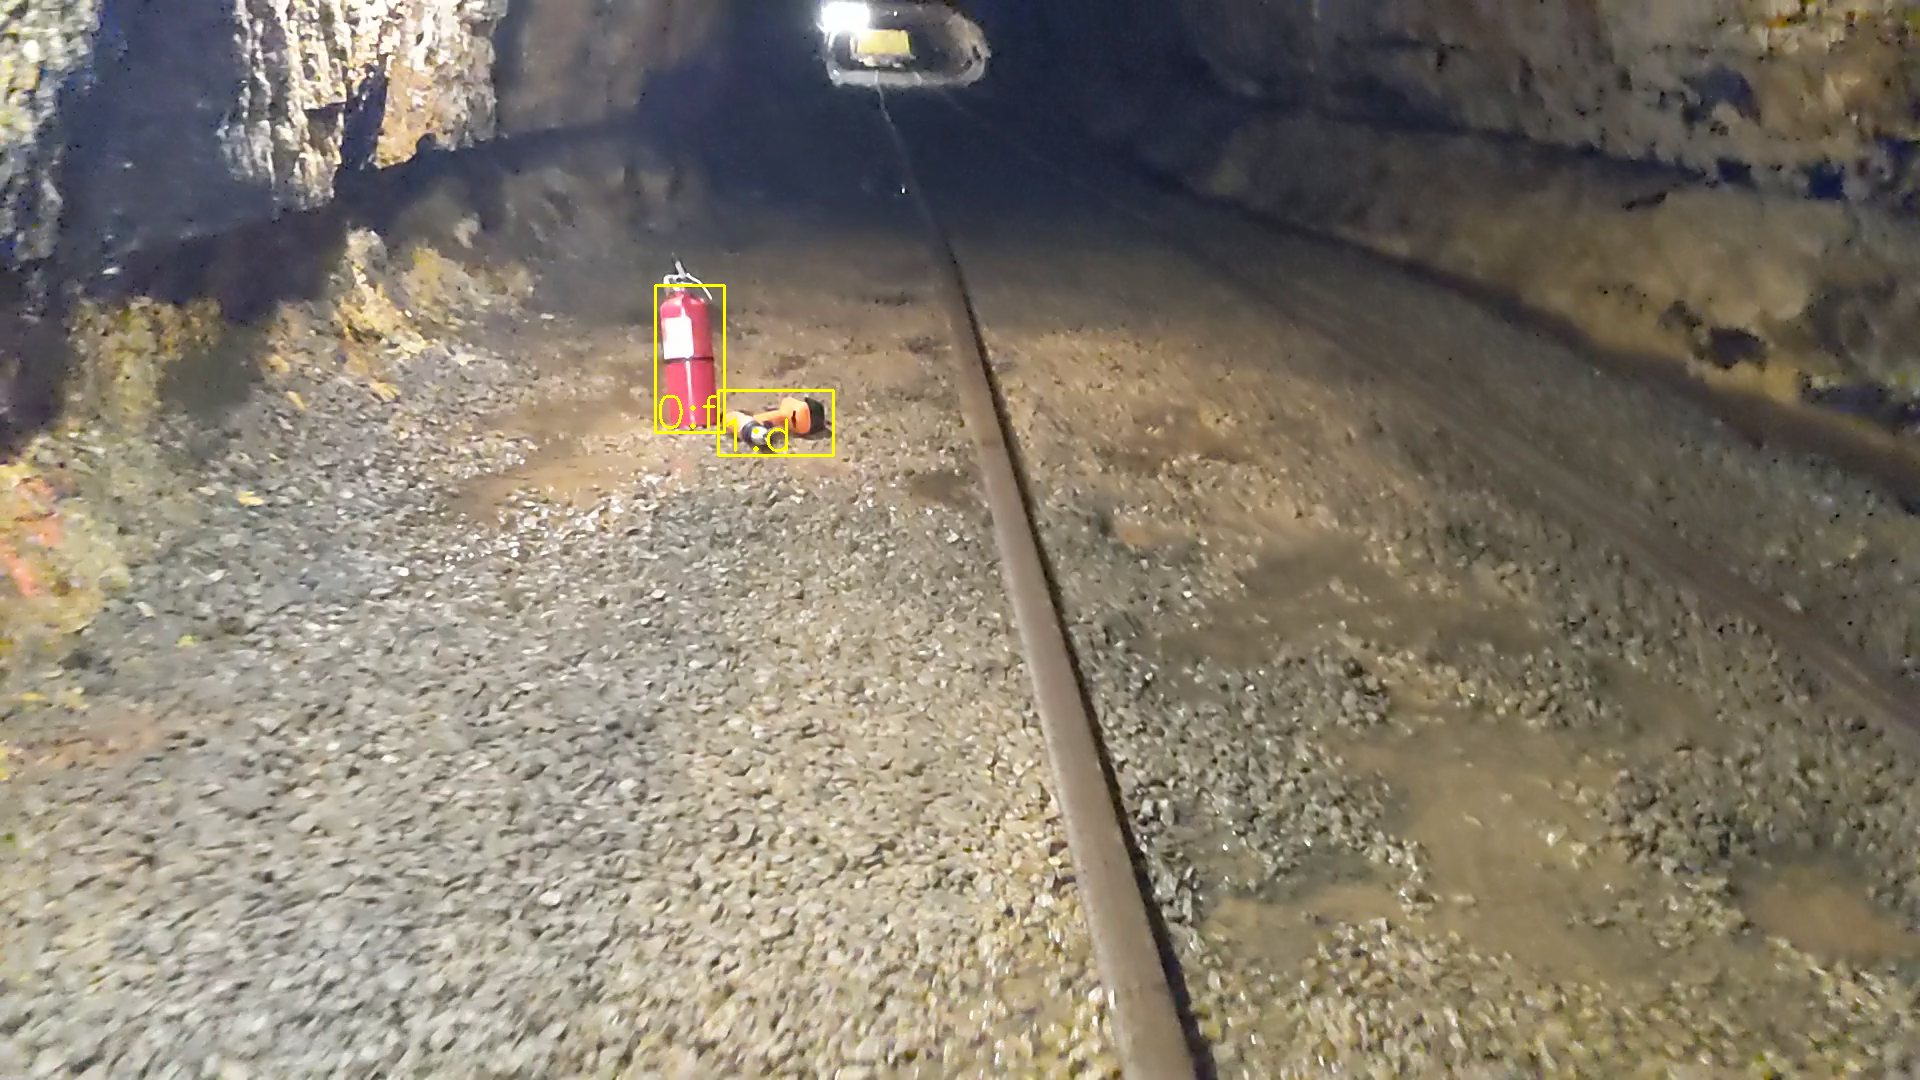
\includegraphics[width=\textwidth]{tracking/rect_00900.png}
	\end{subfigure}	
	\caption[Example video labeled with semi-automatic pipeline]{Example video labeled with semi-automatic labeling pipeline. The number inside the bounding box indicates the ID the artifact in the image (0-indexed), and the letter is a 1 letter identifier for the classification (d for drill, f for fire extinguisher).}
	\label{semi_automatic_labeling}
\end{figure}

A few parameters were added to the labeling program to trade off between labeling accuracy and speed. The tracker performance could be modified with a flag to change the scale of the image used for tracking. Downsampling the image resulted in a faster tracker framerate, but at occasionally reduced quality. The tracker type could also be changed for each video clip. We determined that, of the trackers we considered (those available in the OpenCV contrib library \cite{opencvcontrib}), the CSRT tracker \cite{lukezic2017discriminative} offered the best tracking accuracy while maintaining a reasonable framerate (typically around 30 fps on a laptop) at native resolution, and thus it was used for all labeled video clips. Only every 5th labeled video frame was added to the dataset to reduce redundancy between samples.

The semi-automated labeling pipeline requires the handheld video to be recorded in a specific way to ensure a good tracker initialization, as described in the previous section. Videos recorded from the payloads on each robot do not have the all of the artifacts visible in the beginning and throughout the entire video, and thus and must be labeled manually. To speed up the manual labeling process, a second custom labeling program was developed. Labelers watch the video at an accelerated speed until they see an artifact. They then step backwards in the video until the artifact first entered the frame, and begin labeling every 5th frame. After drawing a box around an artifact (two clicks), the class can be assigned by pressing a single key (unique per class) on the keyboard. The last assigned class is preserved between frames to simplify the common case of only a single artifact being visible in frame. A tracker was not used to propagate labels between frames due to time constraints, but was the labelers' most requested feature. All labeled images, from both the semi-automated and manual labeling programs, were validated by two additional labelers to ensure consistent, high quality labels.

During the labeling process, we discovered the cell phone artifact was particularly difficult to label due to its small size, dark color which did not offer significant contrast to the environment, and large appearance variation due to the video being played on it. We speculated that a neural network would have similar issues when attempting to detect the cell phone, and thus did not label a significant number of cell phones in RGB images during the labeling process.

\subsubsection{Dataset Generation and Statistics}

Not all labeled images were used to train networks for the Tunnel Circuit. The sparse distribution of artifacts in the environment means that the video collected from the robots' payloads will have a large percentage of frames without artifacts, typically larger than 90\% per video. Using such a large number of negative examples negatively impacts training performance and thus many must be filtered out. The train and eval datasets were generated such that there could be no more than a set ratio (15\%) of negative examples to overall examples. Additionally, since all training images were sampled from videos, randomly distributing the videos into a train and eval set would not be sufficient as videos are highly correlated and the resulting sets would be very similar. Instead, entire video clips were manually assigned to be a part of either the train or eval datasets. All images were preserved at their native resolution (640 x 360) and losslessly encoded when added to the dataset. Any labels for cell phone artifacts were discarded. Statistics on the RGB train and eval datasets are presented in Table \ref{rgb_statistics}.

% Tested on 2019-06-07 in tunnel_circuit_dataset by running find . -type f -iname "*.txt" | wc -l and  find . -empty -type f -iname "*.txt" | wc -l

\begin{table}
	\centering
	\begin{adjustbox}{max width=.9\textwidth}
		\csvreader[
		respect underscore=true,
		tabular=|l|c|c|,
		late after line=\\\hline,
		% This is a terrible hack to get the multiline support I want.
		table head=\hline \textbf{Statistic} & \textbf{Train} & \textbf{Eval}\\\hline,
		]{rgb_statistics.csv}{}{\csvlinetotablerow}
	\end{adjustbox}
	\caption{Dataset statistics for Tunnel Circuit RGB Dataset}
	\label{rgb_statistics}
\end{table}
 
\subsection{Training}

All neural network training was performed using the TensorFlow Object Detection API. The benchmarks in Table \ref{trt_graphs} and Table \ref{openvino_graphs} indicated that the MobileNet + SSD family of networks would offer the highest framerates, so a number of configurations using MobileNet were trained. All network configuration files were derived from checkpoint files available in the TensorFlow Object Detection API, with all values except those mentioned left as provided. Each configuration used a batch size of 12, an input image size of 640 x 360, and the random horizontal flip, random brightness adjustment, random contrast adjustment, and ssd random crop data augmentations provided by the API with their default parameters. The RMSProp optimizer was used to train all networks, with a decay of 0.9, a momentum value of 0.9, an epsilon value of 0.9, and an exponentially decaying learning rate with an initial learning rate of 0.004, 500000 decay steps, and a decay factor of 0.95. A score threshold of 0.4 was used for non maximum suppression.

Networks using either MobileNet V1 or Mobilenet V2 as a feature extractor, SSD or SSD Lite as an object detection head, and focal loss or hard example mining as a loss function were trained, resulting in 8 separate configurations. Each network was initialized using checkpoints provided by the TensorFlow Object Detection API, which are pretrained for classification on ImageNet and then trained for object detection on COCO. All configurations were trained for a week with a single GPU for each network on an AWS p3.16xlarge instance. As no limit was placed on the number of steps for each network, checkpoints were kept every 4 hours of training to allow a checkpoint to be selected during evaluation from any point in the training.

\subsection{Evaluation}

COCO evaluation metrics were used to quantify the performance of each network. The overall loss plot for each network (in Figure \ref{rgb_loss}) indicates that each network reached convergence by approximately 300k steps. The COCO metrics for each network configuration at 300k steps are given in Table \ref{rgb_training}. The table indicates that while the SSD Lite MNV2 Focal configuration had the best overall performance, all of the networks performed comparably in the majority of the evaluation metrics. As inference speed was a priority, using guidance from the previous benchmarking results we decided to use the SSD MNV1 Hard configuration for the Tunnel Circuit.

\begin{figure}	
	\centering
	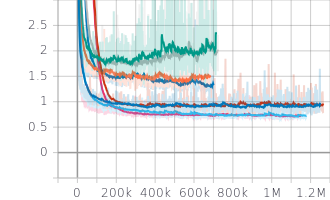
\includegraphics[width=0.45\textwidth]{rgb_loss.png}
	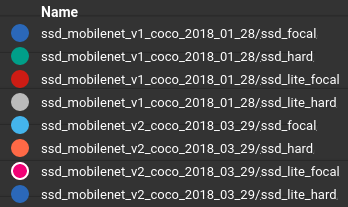
\includegraphics[width=0.45\textwidth]{training_legend.png}
	\caption[RGB network loss values]{Loss values for all 8 configurations, with a smoothing of 0.95 applied in TensorBoard. X axis indicates number of steps. Y axis indicates overall loss value.}
	\label{rgb_loss}
\end{figure}

\begin{table}
	\centering
	\begin{adjustbox}{max width=.95\textwidth}
		\csvreader[
		respect underscore=true,
		tabular=|l|c|c|c|c|c|c|c|c|c|c|c|c|,
		late after line=\\\hline,
		% This is a terrible hack to get the multiline support I want.
		table head=\hline \textbf{Configuration} & \textbf{mAP} & \textbf{mAP$_{large}$} & \textbf{mAP$_{med}$} & \textbf{mAP$_{small}$} & \textbf{mAP$_{0.5 IOU}$} & \textbf{mAP$_{0.75 IOU}$} & \textbf{AR$_{1}$} & \textbf{AR$_{10}$} & \textbf{AR$_{100}$} & \textbf{AR$_{large}$} & \textbf{AR$_{med}$} & \textbf{AR$_{small}$} \\\hline,
		]{rgb_training.csv}{}{\csvlinetotablerow}
	\end{adjustbox}
	\caption[COCO evaluation metrics for RGB networks at 300k steps]{COCO evaluation metrics for RGB networks at 300k steps. MNV1 and MNV2 configurations use MobileNet v1 and v2 feature extractors respectively.}
	\label{rgb_training}
\end{table}

\subsection{Inference}

The selected RGB network is used for inference on each platform by first optimizing it as described in the benchmarking section with either TensorRT or OpenVINO, and then using a custom inference node to feed images through the network. When inferring on images from multiple cameras, batch inference is done on a set of images containing one image from each camera. A list of detected objects is published for each frame, containing bounding boxes, a classification, and a classification confidence. An empty list is published if no objects are detected.

\section{Object Detector (Thermal)}

The development of the thermal object detector closely mirrored that of the RGB object detector. The same data collection and labeling pipeline was used to label thermal images. Thermal images proved more difficult to label, but labelers found that viewing RGB images of the scene alongside the thermal images increased labeling speed. Backpacks, drills, and fire extinguishers were discovered to have minimal thermal signatures and were excluded from labeling. Cell phones were visible in thermal images but proved too small to label accurately and were thus also excluded from labeling. Only the survivor artifact was labeled. All data was kept at the native camera resolution of 640 x 512 and losslessly encoded. The dataset was generated in a similar fashion to the RGB dataset, though no negative examples were used. Statistics for it are given in Table \ref{thermal_statistics}.

\begin{table}
	\centering
	\begin{adjustbox}{max width=.9\textwidth}
		\csvreader[
		respect underscore=true,
		tabular=|l|c|c|,
		late after line=\\\hline,
		% This is a terrible hack to get the multiline support I want.
		table head=\hline \textbf{Statistic} & \textbf{Train} & \textbf{Eval}\\\hline,
		]{thermal_statistics.csv}{}{\csvlinetotablerow}
	\end{adjustbox}
	\caption{Dataset statistics for Tunnel Circuit Thermal Dataset}
	\label{thermal_statistics}
\end{table}

Thermal object detection network training was performed after the RGB network had been trained. Using the insight from training the various RGB network configurations, we decided to only train a single configuration of the thermal network, identical to that of the selected RGB network (SSD MNV1 Hard). All configuration parameters were reused, with the only difference being the dataset. The process for inference with the thermal network is also identical to that of the RGB network.

\section{LIDAR Renderer}

The LIDAR renderer uses camera information (intrinsics and extrinsics) and registered point clouds from LOAM to render depth images. For RGB images, the LIDAR renderer provides an alternative source for depth information as depth images are already produced by the RealSense cameras. However, the LIDAR renderer serves as the only source of depth information for the thermal cameras, as they do not otherwise have associated depth information.

\subsection{Method}

Two implementations of the LIDAR renderer were written - a reference implementation which runs on CPU, and an optimized one which runs on a GPU using CUDA. The optimized implementation is used on both Mk. 0 and Mk. 1 and runs on the Xavier, where it renders depth images for either 5 or 6 image streams (4x RGB and 1 or 2x thermal). The reference implementation was used to validate the GPU implementation for correctness. The reference implementation also runs on the NUC on the drone payload as it does not have a GPU that supports CUDA. The slower performance of the reference implementation is acceptable as renders only need to be produced for a single RGB stream. Both implementations share the same overall algorithm, comprising two separate tasks -- cloud aggregation and rendering.

\subsubsection{Cloud Aggregation}
The renderer aggregates the registered point clouds from LOAM. A rolling buffer of these clouds is maintained, whose size is proportional to the time it takes to render an image. 10 clouds are stored in the reference implementation, and 30 clouds are stored in the GPU implementation. The clouds are already transformed into a common frame and form a locally smooth point cloud. Global drift is present, but can be ignored since the rendered depth images only see a small local portion of the map.

\subsubsection{Rendering}
For each rendered image, the renderer computes the position of the camera in the same frame as the aggregated point clouds. The renderer then uses the camera intrinsics to construct a pinhole camera model and projects each point through it to obtain a location in image coordinates. This coordinate, as well as pixels around this coordinate (based on a configurable inflation parameter) are updated based on the distance to the point, keeping the closer point. The projected coordinates are inflated (as shown in Figure \ref{lidar_inflate}) to provide a denser output image to ensure that depth values are not lost in any potential future downsampling. An inflation value of 4 was used for all payloads.

\begin{figure}
	\centering
	\begin{subfigure}{0.32\textwidth}
		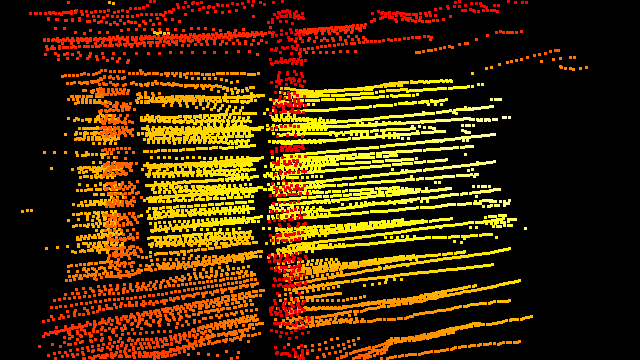
\includegraphics[width=\textwidth]{inflate_1_colormapped.png}
		\caption{1 pixel inflation}
		\label{inflate_1}
	\end{subfigure}		
	\hfill
	\begin{subfigure}{0.32\textwidth}
		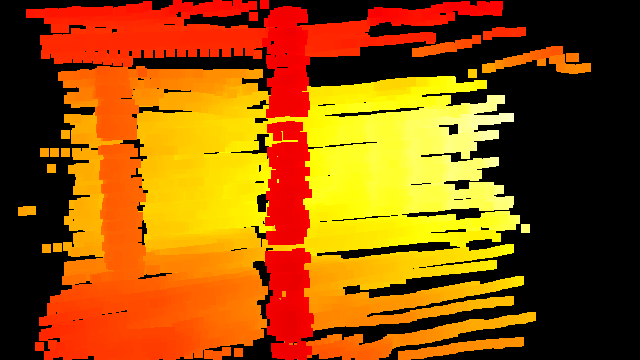
\includegraphics[width=\textwidth]{inflate_4_colormapped.png}
		\caption{4 pixel inflation}
		\label{inflate_4}		
	\end{subfigure}
	\hfill
	\begin{subfigure}{0.32\textwidth}
		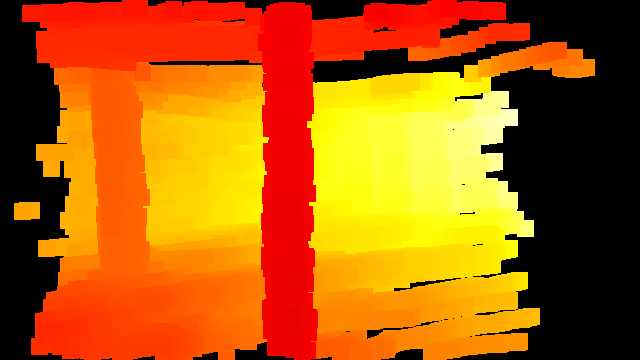
\includegraphics[width=\textwidth]{inflate_8_colormapped.png}
		\caption{8 pixel inflation}
		\label{inflate_8}
	\end{subfigure}
	\caption[LIDAR renderer inflation values comparison]{Rendered images of the same scene with different inflation values. An inflation value of 4 was used for all payloads.}
	\label{lidar_inflate}
\end{figure}

\subsection{Results}

A selection of outputs from the LIDAR renderer running on Mk. 1 is given in Figure \ref{lidar_renderer_images}, along with the depth image output from the RealSense camera and the associated RGB image for reference. In the first row, with Mk. 1's camera looking down a long tunnel, the rendered image is significantly sharper and more consistent than that of the RealSense. In the second row, with the left camera looking at a nearby wall, both depth images are similar. In the final row, with a scene from Mk. 1's back camera (which is tilted upwards), the RealSense depth image has significantly fewer holes than the LIDAR's due to the LIDAR's narrow vertical field of view. 

These results show that the output from the LIDAR renderer is either on par with, or better than that from the RealSense cameras, assuming the camera's full field of view is captured by the LIDAR. By fusing both depth images in the Depth Combiner, we obtain better depth images than either source provides individually.

\begin{figure}
	\centering
	\begin{subfigure}{0.32\textwidth}
		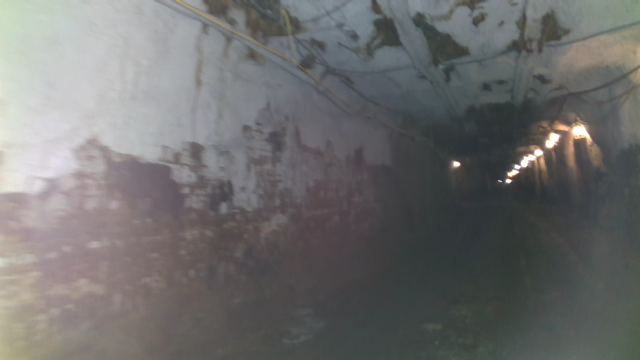
\includegraphics[width=\textwidth]{rs_front_example_2019-10-16-00-51-04_color.png}
		\caption{Mk. 1 Front Color}
		\label{lidar_front_color}
	\end{subfigure}		
	\hfill
	\begin{subfigure}{0.32\textwidth}
		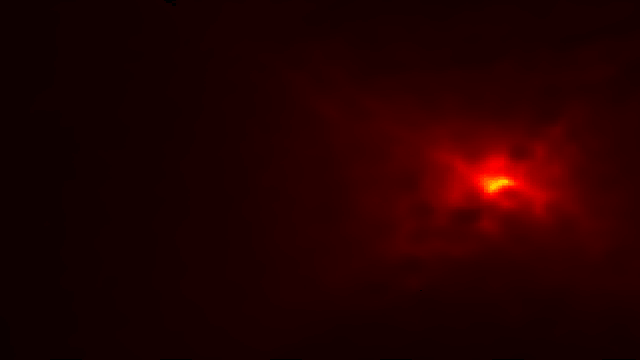
\includegraphics[width=\textwidth]{rs_front_example_2019-10-16-00-51-04_ref_colormapped.png}
		\caption{Mk. 1 Front Depth}
		\label{lidar_front_ref}		
	\end{subfigure}
	\hfill
	\begin{subfigure}{0.32\textwidth}
		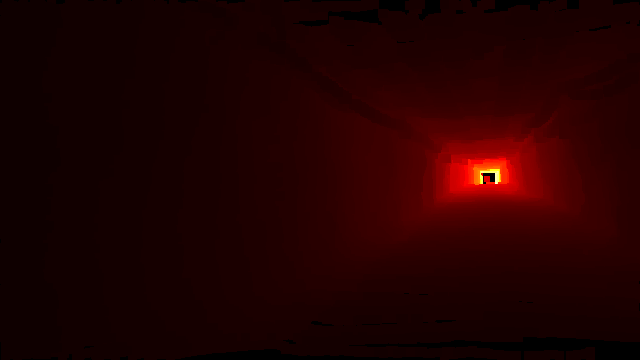
\includegraphics[width=\textwidth]{rs_front_example_2019-10-16-00-51-04_render_colormapped.png}
		\caption{Mk. 1 Front Rendered}
		\label{lidar_front_render}
	\end{subfigure}
	\\
	\begin{subfigure}{0.32\textwidth}
		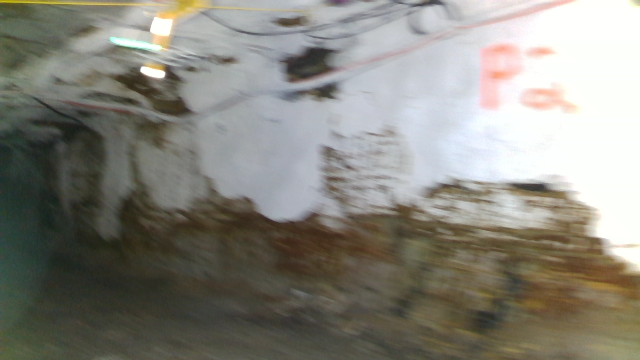
\includegraphics[width=\textwidth]{rs_left_example_2019-10-16-00-51-02_color.png}
		\caption{Mk. 1 Left Color}
		\label{lidar_left_color}
	\end{subfigure}		
	\hfill
	\begin{subfigure}{0.32\textwidth}
		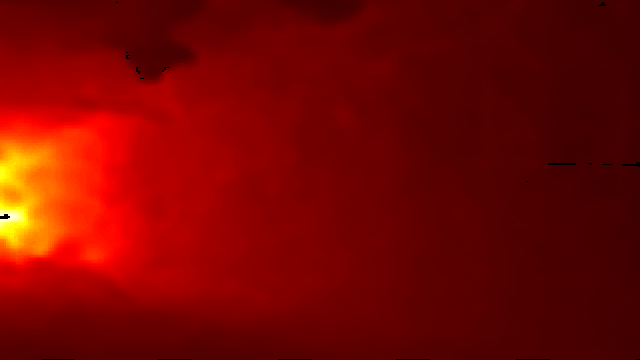
\includegraphics[width=\textwidth]{rs_left_example_2019-10-16-00-51-02_ref_colormapped.png}
		\caption{Mk. 1 Left Depth}
		\label{lidar_left_ref}		
	\end{subfigure}
	\hfill
	\begin{subfigure}{0.32\textwidth}
		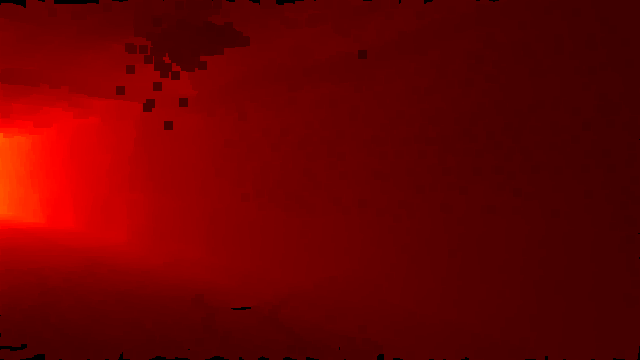
\includegraphics[width=\textwidth]{rs_left_example_2019-10-16-00-51-02_render_colormapped.png}
		\caption{Mk. 1 Left Rendered}
		\label{lidar_left_render}
	\end{subfigure}
	\\
	\begin{subfigure}{0.32\textwidth}
		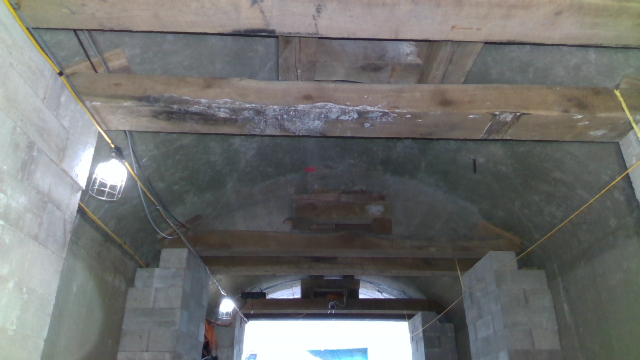
\includegraphics[width=\textwidth]{rs_back_example_2019-10-16-00-33-41_color.png}
		\caption{Mk. 1 Back Color}
		\label{lidar_back_color}
	\end{subfigure}		
	\hfill
	\begin{subfigure}{0.32\textwidth}
		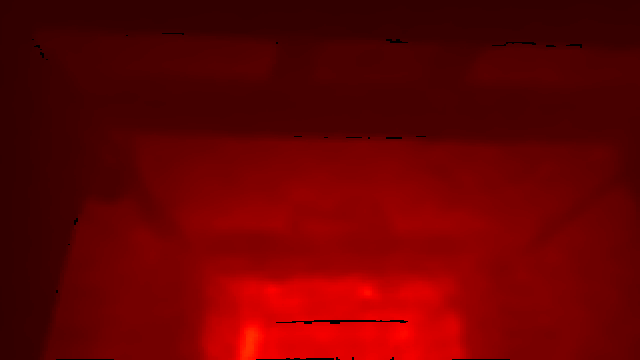
\includegraphics[width=\textwidth]{rs_back_example_2019-10-16-00-33-41_ref_colormapped.png}
		\caption{Mk. 1 Back Depth}
		\label{lidar_back_ref}		
	\end{subfigure}
	\hfill
	\begin{subfigure}{0.32\textwidth}
		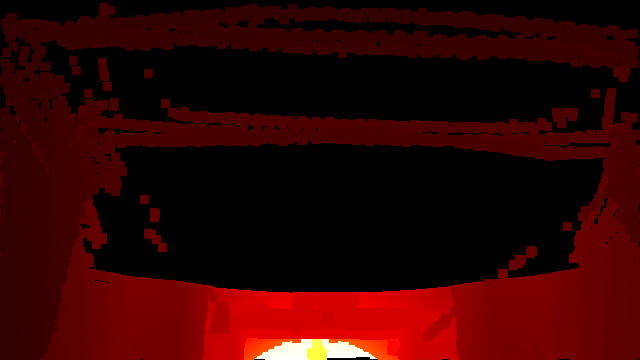
\includegraphics[width=\textwidth]{rs_back_example_2019-10-16-00-33-41_render_colormapped.png}
		\caption{Mk. 1 Back Rendered}
		\label{lidar_back_render}
	\end{subfigure}		
	\caption[LIDAR renderer depth image comparison]{Comparison of depth images generated by the LIDAR renderer to depth images from the RealSense cameras. Color images, captured simultaneously by the RealSense cameras, are provided for reference.}
	\label{lidar_renderer_images}
\end{figure}

\section{Depth Combiner}

The depth combiner fuses depth images from the RealSense depth camera and LIDAR renderer into a single depth image to be used in the object detection localizer. The two image streams are aligned, and can thus be fused per-pixel. The following equation was used (shown as C++ code):

\begin{lstlisting}[language=c++]
fused = (realsense > threshold || realsense == 0) ? lidar : realsense;
\end{lstlisting}

This fusion keeps LIDAR data whenever the reported RealSense data is either not present (\lstinline[language=c++]{realsense == 0}) or exceeds some threshold (\lstinline[language=c++]{realsense > threshold}). The threshold was empirically selected to be 2.5m, which is the approximate distance after which we observed significant variance in reported depth values between frames. This fusion allows us to use the high density RealSense depth information whenever it is available and sufficiently accurate (under the 2.5m threshold), and utilize the sparser LIDAR information otherwise. An example output is given in Figure \ref{combined_depth}.

\begin{figure}
	\centering
	\begin{subfigure}{0.32\textwidth}
		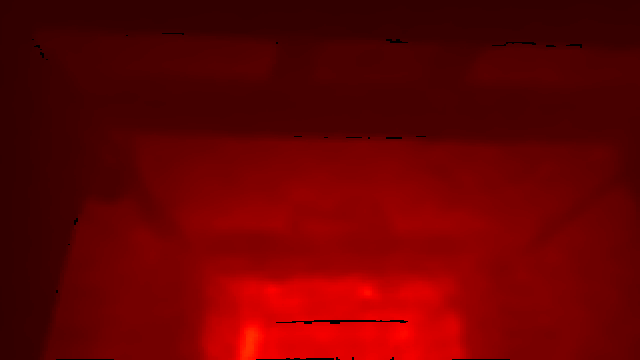
\includegraphics[width=\textwidth]{rs_back_example_2019-10-16-00-33-41_ref_colormapped.png}
		\caption{Mk. 1 Back Depth}
		\label{combined_depth_realsense}		
	\end{subfigure}
	\hfill
	\begin{subfigure}{0.32\textwidth}
		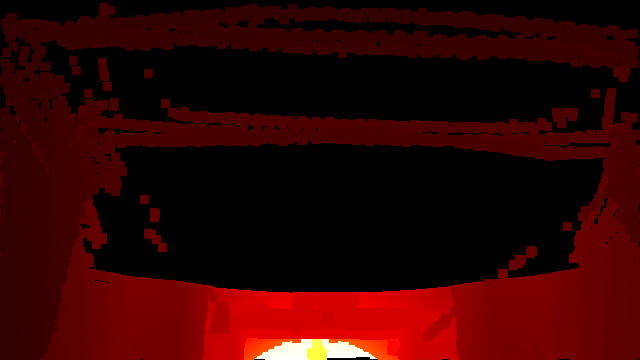
\includegraphics[width=\textwidth]{rs_back_example_2019-10-16-00-33-41_render_colormapped.png}
		\caption{Mk. 1 Back Rendered}
		\label{combined_depth_lidar}
	\end{subfigure}	
	\hfill
	\begin{subfigure}{0.32\textwidth}
		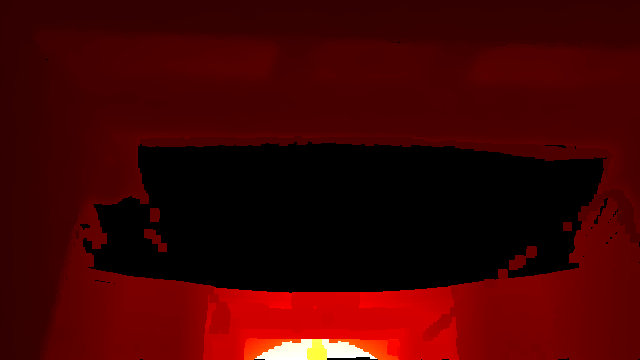
\includegraphics[width=\textwidth]{combined_depth_colormapped.png}
		\caption{Mk. 1 Back Combined}
		\label{combined_depth_output}
	\end{subfigure}		
	\caption[Depth combiner sample output]{Example of the output from the depth combiner, using the same scene as in \ref{lidar_back_color}.}
	\label{combined_depth}
\end{figure}


\section{Object Detection Localizer}

The object detection localizer aggregates multiple 2d object detections for the RGB and thermal images and produces candidate Artifact Localizations. The localizer is able to combine detections of the same object from different camera streams together into a single Artifact Localization. Once sufficient evidence has been obtained for an Artifact Localization, the localizer will publish it to the Artifact Aggregator. Artifact Localizations are updated at 1 Hz using key pose information from LOAM to ensure global correctness for the duration of the robots' exploration. 

For any potential artifact, evidence is only accumulated in the form of positive detections from the object detectors. Negative (empty) detections do not reduce the likelihood that an artifact is present at a given location. This biases the object detection localizer to return a large number of false positives, as most spurious detections from the object detectors will get reported as Artifact Localizations to the base station. This approach is consistent with our requirements and assumptions - as the human supervisor was able to validate artifact reports, even a large number of false positives is acceptable if it means that no artifacts are missed.

The object detection localizer consists of 3 main operations, separated into two threads. The first thread, running the key pose maintenance and detection backprojection tasks, is responsible for creating and maintaining a data structure which stores a 3d point cloud associated with each 2d detection with respect to a key pose. The second thread, running the clustering task, is responsible for extracting new Artifact Localizations from the data structure, updating existing ones, and publishing changes. The clustering task's execution time scales with the size of the data structure and thus runs in a separate thread, allowing all callbacks in the primary thread to be serviced in time.

\subsubsection{Detection Key Pose Maintenance}

The key pose maintenance task is responsible for populating and updating a data structure with key pose information from LOAM. When key poses are initially received, they contain a timestamp and an ID in addition to the pose information. Both pieces of metadata are stored alongside the key pose. The ID is used to update the corresponding key poses when a list of updated key poses is received from LOAM after a loop closure. The timestamp is made available to other tasks to be able to associate other sensor measurements to a key pose.
	
\subsubsection{Detection Backprojection}
The detection backprojection task runs as a callback upon receiving a set of 2d object detections, a color image, an associated depth image, and camera intrinsics information. For each detection, the depth information and camera intrinsics are used to project all pixels which fall inside the bounding box through a pinhole model into a 3d point cloud in the camera frame. The point cloud is colored by the RGB image, and each point in the cloud is assigned an ID corresponding to the classification of the detection. The timestamp of the image frame is then used to look up the immediately preceding key pose in the structure built by the key pose maintenance task. The point cloud is then transformed to be in the key pose's frame, and is added to a list of point clouds associated with that particular key pose. The color image has the bounding box drawn on it, and is stored alongside the point cloud. The centroid of the point cloud is also computed and stored, to enable more efficient clustering. This backprojection process is identical for both RGB and thermal images.
	
It is important that the backprojected point clouds are stored relative to a particular key pose rather than relative to the robot's /map frame to maintain global consistency and handle loop closure events. The transform necessary to convert the point cloud into the key pose frame is obtained in two steps. First, the static transform from the camera to the LOAM sensor frame is combined with the /integrated\_to\_map frame at the image timestamp, yielding a transform from the camera frame to the /map frame. Then, the pose of the corresponding key pose (which is already in the /map frame) is used to create a transform from the camera frame to the key pose frame. Storing the backprojected point clouds relative to a key pose rather than directly in the /map frame allows the clouds to be more accurately transformed into the /map frame as the key poses are updated. By using the /integrated\_to\_map topic, we ensure that the error the eventual transformation into the /map frame is due to small IMU integration error between key poses, rather than a large global drift.
	
Some additional filtering is also performed during this step to improve the quality of data being stored. The robot's pose estimate must move by at least a small amount (7.5cm) between frames, or clouds are not generated at all. This threshold ensures that redundant information does not get stored if the robot is sitting still or moving very slowly. Additionally, depending on the source of depth information being used, different downsampling and depth cutoff parameters are used in the backprojection. Downsampling reduces the density of the backprojected point cloud by skipping certain pixels when backprojecting. Every 4th row and column is kept when utilizing dense RealSense depth information, while every 2nd row and column is kept when using the comparatively sparse LIDAR rendered depth information. The depth cutoff is used to discard any points which have depth values beyond a certain point, and is used to compensate for low accuracy in the depth values. A depth cutoff of 10m was selected, intended to only act as a cutoff for the LIDAR depth values as a lower cutoff of 2.5m was used for the RealSense depth data in the Depth Combiner.
	
\subsubsection{Clustering}
The clustering task continually (at 1 Hz) creates Artifact Localizations from the data structure populated by the backprojection task, and publishes updates for downstream nodes to use. First, the centroid of each backprojected point cloud is transformed into the /map frame using the updated pose of the corresponding key pose. This centroid cloud is then clustered using Euclidean clustering from PCL, with a cluster tolerance of 0.5m and a minimum cluster size of 3. These parameters group objects which have been detected a sufficient number of times (3) and are close enough (0.5m) together. The clustering is purely geometric, and does not account for the classification of the centroid. This choice enables the clustering process to be more robust to misclassification from the network, but in exchange sacrifices the ability to distinguish multiple objects of different types near each other.
	
The centroid of each cluster can be treated as an approximation for the centroid of each artifact that the robot has seen. However, the computed centroid of centroids is imprecise, and can be refined by integrating the complete point clouds for each detection. First, the clouds are transformed into the /map frame and aggregated into a single cloud for the cluster. The centroid of this cloud is then found, and used as the refined position of an Artifact Localization. This centroid differs from the one computed using the centroid of each point cloud as it will weight the centroids based on the number of points in the cloud, rather than weighting all centroids equally. While finding the centroid of the cluster point cloud, a majority vote is performed over the classifications to determine a label for the Artifact Localization. Finally, the color images (with bounding boxes) for each detection in the cluster are added to the Artifact Localization as evidence.
	
Once the complete list of Artifact Localizations has been created from the available data, it is compared against existing valid Artifact Localizations generated by previous iterations. New Artifact Localizations are matched pairwise against previous ones, again only considering Euclidean distance, using a threshold of 0.25m. Previous Artifact Localizations which are matched to new ones have their parameters updated with the ones of their match. Previous ones which were not matched are now considered invalid, and are marked as such, but are not forgotten. New Artifact Localizations which did not match any previous ones are given a new ID and stored as new valid Artifact Localizations. All changes to Artifact Localizations (updates, invalidations, and new ones) are published, along with the IDs of each Artifact Localization. This process of publishing deltas in the list of Artifact Localizations is used to increase memory efficiency and reduce transmission bandwidth, and is used everywhere Artifact Localizations are published.
	
When publishing Artifact Localizations, only a small number of images are kept. Typically, an Artifact Localization will amass 50 or more detections from different cameras as the robot drives by an artifact. These images are highly redundant, and it is thus inefficient to transmit them all. Instead, only 4 selected images are published. The images are sorted by their capture timestamp and then evenly distributed into 4 chunks. The first image from each chunk is kept, resulting in images which show multiple perspectives of an artifact as the robot travels by. An example of 4 automatically selected images for an artifact is shown in Figure \ref{automatically_selected_images}.

\begin{figure}
	\centering
	\begin{subfigure}{0.45\textwidth}
		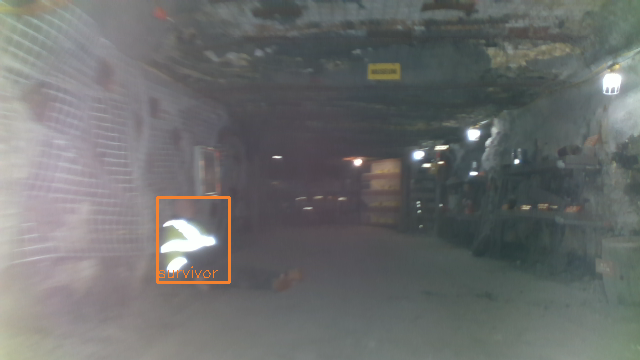
\includegraphics[width=\textwidth,height=4cm,keepaspectratio]{artifact_0019_image_00.png}
		\caption{Survivor Image 1}
		\label{survivor_image_1}
	\end{subfigure}		
	\hfill
	\begin{subfigure}{0.45\textwidth}
		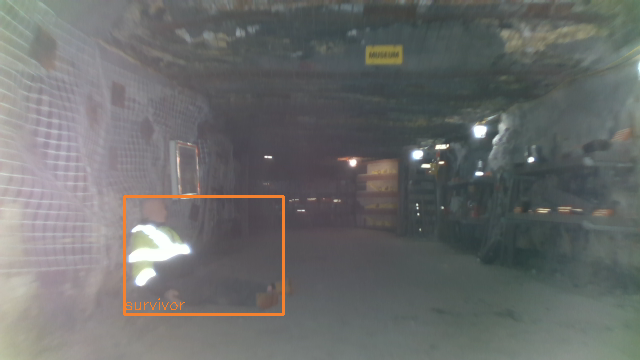
\includegraphics[width=\textwidth,height=4cm,keepaspectratio]{artifact_0019_image_01.png}
		\caption{Survivor Image 2}
		\label{survivor_image_2}
	\end{subfigure}
	\\
	\begin{subfigure}{0.45\textwidth}
		\centering
		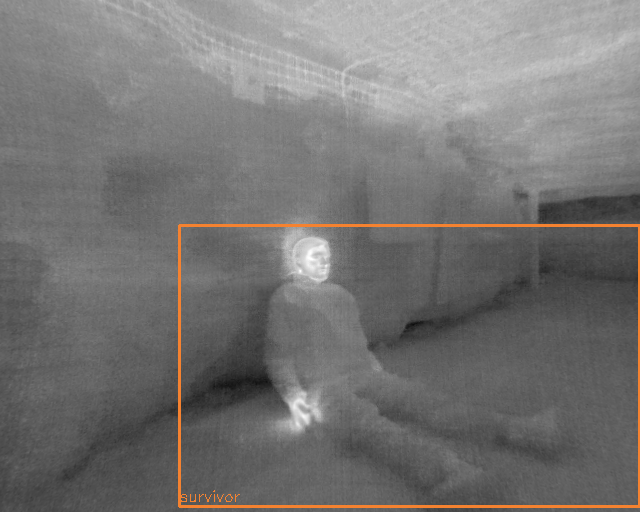
\includegraphics[width=\textwidth,height=4cm,keepaspectratio]{artifact_0019_image_02.png}
		\caption{Survivor Image 3 (thermal)}
		\label{survivor_image_3}
	\end{subfigure}
	\hfill
	\begin{subfigure}{0.45\textwidth}
		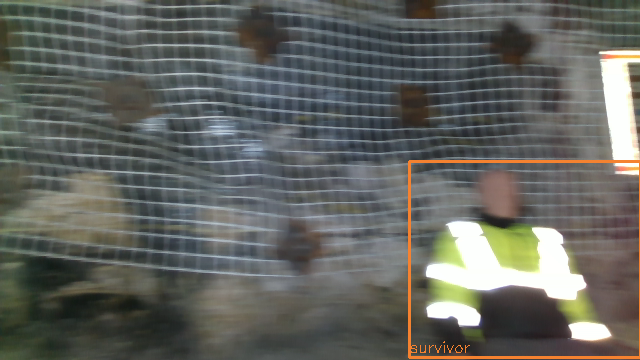
\includegraphics[width=\textwidth,height=4cm,keepaspectratio]{artifact_0019_image_03.png}
		\caption{Survivor Image 4}
		\label{survivor_image_4}
	\end{subfigure}		
	\caption[Automatically selected images from Artifact Localizations]{Each published Artifact Localization contains only a few images automatically selected from the many detections which combine together to form a single Artifact Localization. These images can be selected across different cameras and different types of cameras, as shown above.}
	\label{automatically_selected_images}
\end{figure}

\section{WiFi Scanner}

The WiFi scanner uses the WiFi modules on the NUC (Mk. 0, Mk. 1, drone) and the Xavier (Mk. 1) to search for nearby devices acting as access points. Scans are run using wpa\_supplicant and are run continuously. Each scan produces a list of nearby access points with a MAC address, SSID (if available), and an RSSI value. The scan results are timestamped with the completion time of the scan, are assigned a frame ID coincident with the LOAM sensor, and are published immediately. Each scan takes approximately 3 seconds to complete, and thus Mk. 0 and the drone payloads publish scan results at approximately .35 Hz while Mk. 1 is able to publish at approximately double the rate, between 0.6 - 0.8 Hz since it uses two WiFi chips to scan instead of just one. Other WiFi interfaces are present on each robot, but are used for wireless communication. The process of WiFi scanning significantly reduces the available bandwidth for wireless communication and thus the WiFi scanner is only allowed to use interfaces which are otherwise unused.

\section{Signal Localizer}

The signal localizer produces Artifact Localizations for cell phone artifacts using the scan results from the WiFi scanner. A Bluetooth scanner was also implemented that could feed into the signal localizer, but was disabled due to low reliability. The structure of the signal localizer is quite similar to that of the object detection localizer. Artifact Localizations are generated continually at 1 Hz, and are updated with new key pose information when available. When changes to the Artifact Localizations are significant, they are published to be used downstream.

Like the object detection localizer, the signal localizer consists of 3 main operations, this time running in a single thread. The first two tasks maintain a data structure with key pose information and wifi scan results. The third task continually solves for positions of cell phone artifacts based on the scan results, and publishes Artifact Localizations for new detections or for significant position changes.

\subsubsection{Signal Key Pose Maintenance}

This task is functionally equivalent to the key pose maintenance task in the object detection localizer. Key poses are stored in a data structure alongside their timestamp and ID, and are updated with new poses from loop closures when available.

\subsubsection{Signal Reading Storage}

This task serves a similar role to the object detection localizer's detection backpropagation task - to populate a data structure with sensor data to be used by a solver. DARPA guarantees that each cell phone artifact's access point will have an SSID of the form "PhoneArtifact\#\#", where \#\# is non-negative 2 digit integer. The scan result is filtered to remove all SSIDs which do not match the provided pattern. All remaining results are guaranteed to belong to a distinct cell phone artifact. Using the timestamp of the scan result, the robot's sensor frame position is determined relative to the nearest key pose, in a manner similar to that in the object detection localizer. The transformation between the robot's sensor frame and the antennas is ignored. Each remaining scan result, consisting of a MAC address, SSID, and RSSI value, is stored with the robot's computed position relative to the corresponding key pose in the data structure.

\subsubsection{Signal Localization} 

Each cell phone artifact has a unique MAC address, which allows multiple readings for the same cell phone artifact to be aggregated together. Readings are gathered by MAC address and each group is processed sequentially in an identical manner. First, the stored position (which is relative to a key pose) is transformed to the robot's /map frame using updated key pose information. This creates a list of RSSI values at different locations, which is the setup for typical cell phone trilateration problems. However, treating the cell phone localization problem as one of trilateration requires a model to convert from RSSI to distance. While these models work well with line of sight between the transmitter and receiver, we were unable to obtain accurate distance estimates around multiple corners and through thick rock walls, and thus an alternate solution was implemented.
	
The alternate solution relies on an important insight about the structure of the problem. We realized that the corridors in the tunnel circuit are quite narrow, meaning that the robot would, at some point, get within a meter or two of each artifact as it drove by them. Since the maximum allowable error for artifact positions was 5m, simply reporting the position of the robot with the highest RSSI value for each cell phone could be sufficient, using the assumption that RSSI was inversely proportional to the robot's distance from the artifact. This is the case for RSSI values from WiFi scanning, but is not true for Bluetooth. Results from Bluetooth scans would saturate the RSSI value when the robot was within approximately 20m of the cell phone, requiring a slightly more complex solution than simply finding the largest RSSI value.
	
First, the received RSSI values and corresponding robot poses are sorted by timestamp. Then, the highest RSSI value is found, and the list of RSSI values is segmented into contiguous groups where the RSSI values equal the maximum found. For WiFi, the maximum RSSI value will typically only occur for one  reading, so the corresponding pose can be returned immediately. For Bluetooth, the groups are typically a set of values for each time the robot drove by the cell phone (e.g. going into and coming out of the tunnel) since the RSSI readings saturate when within 10m to 20m of the cell phone. The midpoint of the arc formed by the robot poses in each set is then found. The midpoints for each set are averaged together and reported as the position of the cell phone artifact. After positions are determined for each cell phone artifact, they are compared against those from the previous iteration, and updates are published in a manner similar to the object detection localizer if any new cell phones are present, or if any have moved significantly.


\section{State Estimate Delay Estimator}

An implementation detail of LOAM is that the timestamps for the state estimates are based on a separate clock than other connected components. Subsecond precision for this clock comes from the IMU's internal clock, which starts counting from 0 at the IMU's startup, while the seconds count is derived from the NUC's system time. This scheme results in an offset between the two clocks of between 0 and 1 seconds, with the NUC's system clock always being ahead. This offset is different with each initialization of the state estimation system, but is consistent for the duration of a run (1 - 2 hours). All other clocks on a robot are synchronized to the NUC's system clock using Chrony, which results in an error on the order of hundreds of microseconds between clocks and is considered negligible.

The state estimate delay estimator estimates the offset between the NUC's system clock and the state estimate clock and publishes the offset to be used by other nodes which use data from both the state estimate and other sensors. Subscribers subtract the published estimate from the timestamp of received sensor data when querying the robot or sensor pose corresponding to sensor data. The estimate is obtained by computing a moving average of the offset between the published timestamp and the NUC's system time for every twentieth state estimate received on the 200 Hz /integrated\_to\_map topic. The estimate is published every update, resulting in a rate of 10 Hz. The following equation is used to update the estimated delay:

\begin{equation} \label{delay_estimate_equation}
d_{now} = 0.9 \ d_{prev} + 0.1 \ (t_{now} - t_{state})
\end{equation}

where $d_{now}$ is the current delay estimate, $d_{prev}$ is the previous estimate (initialized to 0), $t_{now}$ is the current system time, and $t_{state}$ is the timestamp contained in the state estimate. An example output from this filter is shown in Figure \ref{multiple_delays}.

\begin{figure}	
	\centering
	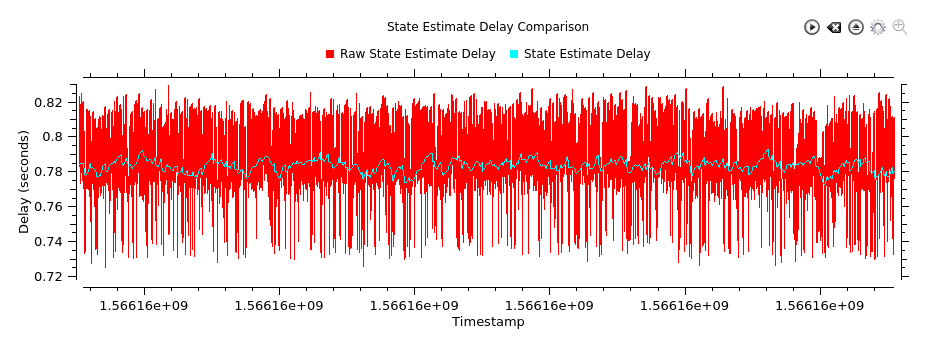
\includegraphics[width=\textwidth]{multiple_delays_screenshot.png}
	\caption[Raw and filtered state estimation delay]{The plot shows delay estimates over a period of 60 seconds from a single run using the Mk. 1 payload. The red line shows the raw delay between the state estimate timestamp and the system time, $t_{now} - t_{state}$, at 200 Hz. The cyan line shows the filtered output using Equation \ref{delay_estimate_equation}, published at 10 Hz.}
	\label{multiple_delays}
\end{figure}

\section{Artifact Aggregator}

% TODO: Link to metrics about lower accuracy
The artifact aggregator combines Artifact Localizations from multiple sources into a single stream using two tasks. 

\subsubsection{Delta Listener}

For efficiency, each source publishes Artifact Localizations as a series of deltas, rather than publishing the entire list of Artifact Localizations at each update. This task listens to the deltas from each source and accumulates them into a complete list of Artifact Localizations for each source. Unlike previous steps in the pipeline, no transformations between frames happen here as the individual sources are expected to publish artifacts in the /map frame and update via deltas when necessary.

\subsubsection{Filtering} 

Every second, the accumulated Artifact Localizations from each stream are combined using a similar clustering mechanism to the object detection localizer. First, the position of each Artifact Localization will be added to a point cloud. No transformation is necessary as all points are already in the /map frame. Then, the point cloud is clustered using PCL's Euclidean clustering with a cluster tolerance of 0.5m and a minimum cluster size of 1. The cluster tolerance was kept the same as the object detection localizer, but the minimum cluster size was reduced to 1 to not ignore any artifacts reported by any source.
	
Artifact Localizations are combined based on their geometric clustering results. For each cluster, the classification of the new Artifact Localization is determined by summing the reported confidence from each constituent Artifact Localization and selecting the class with the highest confidence. The images for the new Artifact Localization are selected identically to the object detection localizer -- all images are sorted, and then 4 images are selected by choosing the first image in each fourth of the list. Individual images may come from different sensing modalities. An example is shown in Figure \ref{automatically_selected_images}. The list of new Artifact Localizations is compared to the previous list of Artifact Localizations to determine a delta (consisting of updates, invalidations, and new Artifact Localizations), which is published and transmitted to the base station.
	
\section{Artifact Debouncer \& Compressor}

The artifact debouncer \& compressor is responsible for providing an efficient and reliable transmission mechanism for Artifact Localizations over the wireless communication link between each robot and the base station. Artifact Localization deltas from the artifact aggregator are used to generate a complete list of Artifact Localizations, each of which is initially marked as dirty. A number of strategies, outlined below, are used to determine which dirty Artifact Localizations should be transmitted to the base station. The bandwidth usage with the various techniques over an hour long competition run from the Tunnel Circuit for Mk. 1 can be seen in Figure \ref{bandwidth_usage}.

\subsubsection{Compression}
The images associated with each Artifact Localization are compressed before transmission. JPEG compression with a quality parameter of 95 is used for each image, resulting in images which are typically between 5 and 10 percent of the original image size in bytes. No other data associated with the Artifact Localization is compressed as its size (10s of bytes) is negligible compared to even the compressed images (each 50-100 kilobytes).
	
\subsubsection{Retransmission} 
The lossy nature of the wireless communication link means that it is not guaranteed that transmitted packets will arrive at the other end. Thus, simply publishing a dirty Artifact Localization is insufficient to guarantee receipt at the base station. This is solved by attaching a timestamp to each transmission and having the receiving node at the base station publish an acknowledgment indicate that it received the Artifact Localization(s) sent at a particular timestamp. Upon receiving this acknowledgment, this node clears the dirty bit from each transmitted Artifact Localization if it was not updated since transmission. This acknowledgment may be dropped when sent via the wireless link as well. This is counteracted by retransmitting dirty Artifact Localizations from each robot until an acknowledgment is received.
	
\subsubsection{Backoff}
One reason for packets not reaching the base station may be that the robot is simply out of wireless communication range. Continually retrying transmission of dirty Artifact Localizations while out of communication range simply pollutes the wireless spectrum for other robots which may still be in range. Thus, linear backoff is employed. After each transmission attempt, an increasing predetermined time must pass before the dirty Artifact Localization can be transmitted again. The delay values are 5, 10, 15, 20, 25, and 30 seconds. Each transmission attempt increases the delay before the next transmission, up to a maximum of 30 seconds.
	
\subsubsection{Debounce}
As a robot drives by an artifact, the artifact will be detected in multiple consecutive camera frames. The object detection localizer will continually update the position of the artifact, and will publish updates every second while the robot drives by. The signal localizer does the same thing as the robot approaches a cell phone. These updates propagate through the artifact aggregator and result in a large number of updates published as the system converges on an estimate of the artifact's location and class. Forwarding each of these updates directly to the base station would be wasteful as another update would follow a second later. This node debounces artifact updates by only marking Artifact Localizations as dirty once an update has not been received for at least 3 seconds. This typically happens after the robot has finished driving by the artifact and can no longer sense it, and is unlikely to update the Artifact Localization again.
	
\subsubsection{Grouping}
Various factors, such as a loop closure event, can result in a large number of dirty Artifact Localizations that are ready to be transmitted. Towards the end of a robot's run, this can be close to 200 Artifact Localizations to transmit at once, or approximately 50 MB assuming an individual compressed Artifact Localization is 250 KB. Sending this much data in a single transmission is infeasible over a wireless link. Instead, a maximum of 10 dirty Artifact Localizations are transmitted at once.
	
\begin{figure}	
	
	\centering		
	%		\begin{subfigure}{\textwidth}
	%			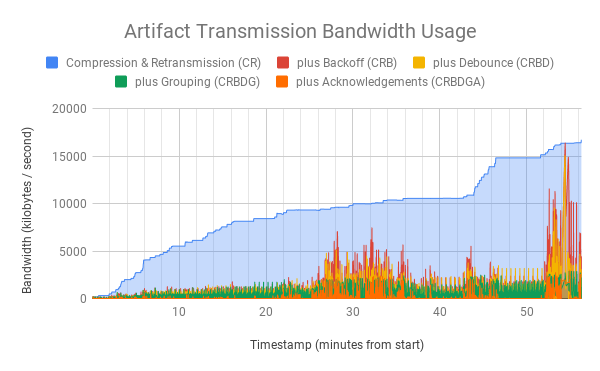
\includegraphics[width=\textwidth]{bandwidth_usage_full.png}
	%			\caption{All bandwidth usage}
	%			\label{bandwidth_usage_full}
	%		\end{subfigure}
	%		\\
	%		\begin{subfigure}{\textwidth}
	%			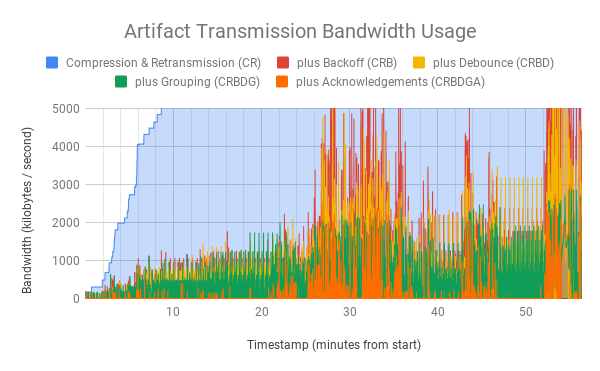
\includegraphics[width=\textwidth]{bandwidth_usage_zoomed.png}
	%			\caption{Bandwidth usage (zoomed)}
	%			\label{bandwidth_usage_zoomed}
	%		\end{subfigure}
	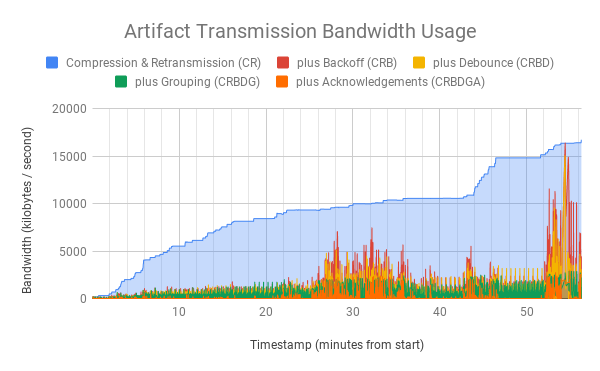
\includegraphics[width=\textwidth]{bandwidth_usage_full.png}
	\caption[Artifact transmission bandwidth usage]{The graph shows the bandwidth used by the compressor to try to transmit artifacts over an hour long competition run from Mk. 1 during the Tunnel Circuit. Features are incrementally added, starting with compression and retransmission, and then backoff, debounce, and grouping. None of these configurations have acknowledgements coming back from the base station, which is common when the robot is not within communication range of the base station. The final configuration (CRBDGA, orange) shows the effect of simulating guaranteed acknowledgements.}
	\label{bandwidth_usage}
\end{figure}


\section{Artifact Uncompressor}

The artifact uncompressor is responsible for receiving and uncompressing Artifact Localization messages sent by the artifact compressor nodes on each robot. Upon receipt of a message, the uncompressor will publish an acknowledgement with the transmission timestamp contained inside the received Artifact Localization message. The acknowledgement is only published once. If the acknowledgement is dropped in transit over the wireless link, the compressor will simply publish the artifact again at a later time. The uncompressor does not manipulate or store the messages it receives in any way - each compressed Artifact Localization received from the compressor node is simply uncompressed and broadcast on the base station for other nodes, such as the GUI, to use.

\section{GUI}

The GUI is used by the human supervisor at the base station to perform a large variety of tasks related to initializing and controlling the fleet of robots. One of these tasks is to validate and, if necessary, refine Artifact Localizations returned from robots in the fleet. Validated Artifact Localizations are reported to DARPA for scoring. An example of the validation GUI, populated with Artifact Localizations, is shown in Figure \ref{gui}. All other tasks performed at the base station are unrelated to the scope of this work.

\begin{figure}
	\centering
	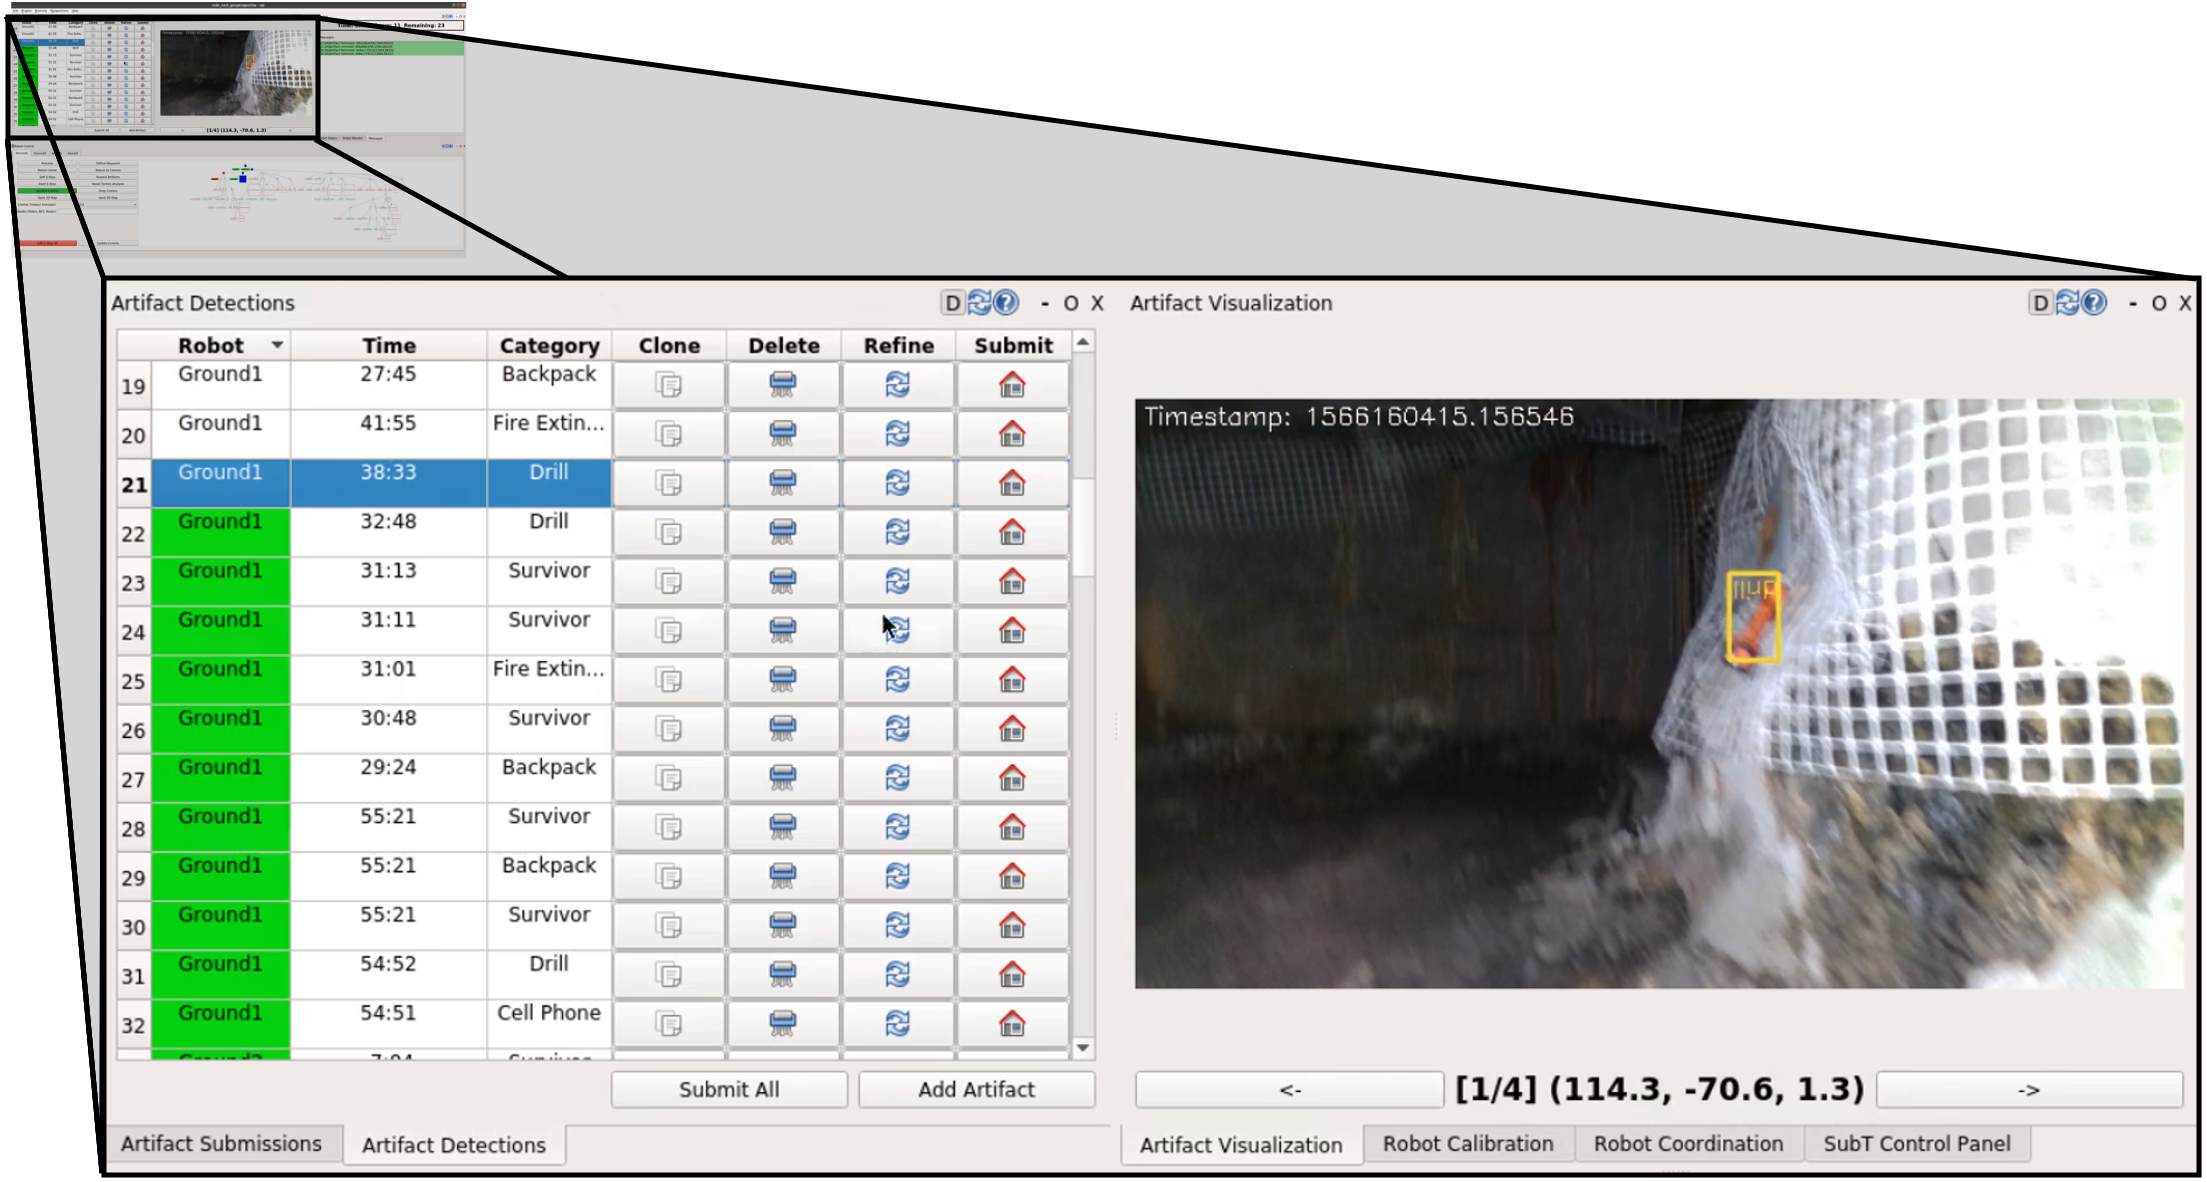
\includegraphics[width=\textwidth]{gui_drill_zoom.png}
	\caption[GUI used for artifact localization validation]{The top left portion of the GUI is used for Artifact Localization verification and consists of two separate panes. The left side of the image shows a queue for Artifact Localizations which still need to be reviewed by the human supervisor, along with the classification and which robot reported the Artifact Localization and when it was detected relative to the start of the run. The right side of the image shows the images contained in the Artifact Localization report, if any, one at a time. The images can be cycled through using the arrows. The coordinates in the Artifact Localization displayed underneath the images.}
	\label{gui}
\end{figure}

Uncompressed Artifact Localizations sent by the artifact uncompressor are received by the GUI and have their coordinates transformed into the DARPA frame using the corresponding robot's calibration. The ID of each Artifact Localization is used to determine whether the Artifact Localization is already being displayed or if a new Artifact Localization has been received. New ones are added to a queue of Artifact Localizations which still need to be inspected by the human supervisor and are highlighted in green. Updates to existing Artifact Localizations either cause them to be removed from the queue, in the case of an invalidation, or simply updated, in which case they will again be highlighted in green. The human supervisor can click on any pending Artifact Localization in the queue, which will render it in white and display the first contained image, if any, and perform one of the following actions:

\begin{enumerate}
	\item \textbf{Submit} -- After verifying that the images, if any, contain an object, that the bounding box is correct, and that the classification matches the object, the Artifact Localization can be submitted to DARPA. If the artifact is within 5m of DARPA's surveyed coordinates, the displayed score in the GUI will increase.
	\item \textbf{Refine} -- If the human supervisor has verified that images, bounding box, and classification are correct and submitted the artifact to DARPA but did not receive a score increase, the artifact position can be manually refined. This can be used to correct for map drift or a poor initial calibration between the robot's world frame and the DARPA frame. The Artifact Localization's class can also be updated if necessary.
	\item \textbf{Clone} -- Any Artifact Localization can be duplicated, with the copy being placed in the queue as a new artifact. This is useful if two artifacts have accidentally been clustered together. The duplicated artifact can be amended manually to match the second of the two artifacts seen in the images.
	\item \textbf{Delete} -- The human supervisor can choose to delete any artifact. Typically, they will delete false positive Artifact Localizations, duplicates from multiple robots, and updates to artifacts which have already been successfully scored.
\end{enumerate}

During the Tunnel Circuit competition event, the human supervisor for Team Explorer was able to inspect approximately 200 Artifact Localizations in less than 5 minutes. Many of these Artifact Localizations could be rejected in less than 1 second due to the displayed image being wrong. Valid Artifact Localizations were submitted quickly in the beginning as no duplicates were possible. Towards the bottom of the queue, additional care was taken to ensure duplicates did not get submitted, increasing the time spent per artifact. Cell phone Artifact Localization coordinates were occasionally refined due to the high error of the signal localizer. No other artifact types were refined unless the human supervisor suspected large map drift had occurred. There were no instances under which the classification of the artifact needed to be updated manually.